%! suppress = FileNotFound
\documentclass[a4paper,12pt]{report}
\usepackage{graphicx}
\usepackage{hyperref}
\usepackage{float}
\usepackage{makecell}
\usepackage[nottoc]{tocbibind}


\pagestyle{headings}
\graphicspath{{./Images/}}
\hypersetup{
	colorlinks=true,
	linkcolor=blue,
	filecolor=magenta,
	urlcolor=cyan,
}


\begin{document}


\begin{titlepage}
	\begin{center}
		\vspace*{1cm}

		\Huge
		\textbf{Design Document - DD}

		\vspace{0.5cm}
		\large
		January 2021

		\vspace{1.5cm}


		\vfill

		
\includegraphics[scale=0.7]{PolimiLogo}

		\vfill


		\normalsize
		\textbf{KONG XIANGYI} \\
		\textbf{\&} \\
		\textbf{ZHANG YUEDONG}

	\end{center}
\end{titlepage}

\tableofcontents


\chapter{INTRODUCTION}\label{ch:introduction}


\section{Purpose}
The purpose of this document is to explain how we design and build CLup application. We demostrate the architecture design of the system, based on the rule of Top-down design approach, we describe the different design characteristics. We explain it from the view of component, deployment and runtime. To be more specific, we also show the user interface design to illustrate the CLup application step by step. The purpose of interface design is user-friendly and efficiently. Our aim is to let other stakeholders can easily understand and know the structure of CLup application.


\section{Scope}
Clup is an application aiming to help user reduce the risk of store in the situation of COVID-19. The user need to have the smart phone to book the ticket. Users or need to take the ticket from the ticket machine out of the store. Users need to scan-in and scan-out when they enter the shop and exit the store. Click customer need to specific their desired product when they booking the ticket. User need to follow the ticket route when they shopping. The manager need to monitor the density of store, control the enter number and reschedule the ticket when too many people in the store or in the same zone. After the click customer insert their information, the system need to design the shopping route for users.


\section{Definitions, Acronyms, Abbreviations}
\subsection{Definitions} \label{subsec:definitions}
\begin{itemize}
	\item Click Customer : The customer has the required technology to access the store.
							I.e a smartphone.
							They can use the customer terminal software.
	\item Brick Customer : The customer doesn't have the required technology to access the store, they have to hand out "tickets" on the spot.
	\item Store Manager : They have to manage the Store System, include the software and hardware.
	\item Ticket: The ticket is a document which contains three key information: QR Code, the estimated departure time, the queue number, and the Store Planned Roadmap.
					To the click customer, it's \textbf{E-ticket} but to the brick customer,it's \textbf{Paper Ticket},and doesn't contain the estimated departure time, and just a General Store Map without the Planned Road.
	\item QR Code : When customer booked a visit, they will received a QR Code.
	\item QR Code Scanned Machine : A hardware, the Click Customer can use this machine scan their QR code.
	\item Tickets Hand-Out Machine : A hardware, the Brick Customer can use it retrieve their Ticket.
	\item Store Planned Roadmap: A store map that includes a finer way which is recommended form Store System.
	\item Digital Counterpart : A hardware, it with show the queue number.
	\item Store Back-End System : A software, as the back-end manages all stuffs.
	\item On-Time Store Data : A dataset that includes the store's on-time date.
	\begin{itemize}
		\item The current queue
		\item The customers in the store
		\item The maximum number of people in the store.
	\end{itemize}
	\item Long-Term Customers: The Click Customer who visited the store more than one time by the CLup mobile application.
\end{itemize}


\subsection{Acronyms}
\begin{itemize}
	\item RASD - Requirement Analysis and Specification Document
	\item DD - Design Document
	\item CLup - Customers Line-up
	\item UI - User Interface
	\item IOS - iPhone OS
	\item PC - Personal Computer
	\item IaaS - Infrastructure as a Service %TODO delete IaaS
	\item CRM - Customer Relationship Management
	\item LAN - Local Area Network
	\item RAPS - Reliable Array of Partitioned Service
	\item RACS - Reliable Array of Cloned Services
	\item MVC - Model-View-Controller
\end{itemize}


\subsection{Abbreviations}
\begin{itemize}
	\item  $R_n$ : n-th functional requirement
	\item  $NR_n$: n-th non functional requirement
	\item  $G_n$ : n-th goal
	\item  $D_n$ : n-th domain assumption
	\item  $C_n$ : n-th component
\end{itemize}


\section{Revision history}


\section{Document Structure}
Here are the structure of DD document:~\\

\textbf{Architectual Design}
In this chapter, we describe the architectural design from the view of component, deployment and runtime. We use the Top-down approach. After we specific the component interfaces. We adopted the 3-Tirered architecture style for our system. We also adopt the relational database.~\\

\textbf{User Interface Design}
Here we illustrated the user interface from the view of user and manager. We have presented some main UI designs in RASD document, here we describe some of them in details. On the end, we use the UX diagram to show the user process.~\\

\textbf{Requirements traceability}
In this chapter, we describe goals with respect to RASD. We specific the corresponding requirements, domain assumptions and components.~\\

\textbf{Implementation, integration and test plan}
In this chapter, we introduce the implementation and integration of different components. After, we did the test of them.



\chapter{ARCHITECTURAL DESIGN}\label{ch:architectural-design}

In this chapter, we will describe the architectural design of our system.

We will use the Top-down design approach, design the very high-level structure first,
and then gradually work down to detailed decisions about low-level constructs.
Finally, arrive at detailed decisions.\cite{SlidesSE2}
Let us start with the High-level components and their interaction.


\section{Overview: High-level components and their interaction}\label{sec:ArchitectureOverview}

We chose \textbf{3-Tiered architecture} with the \textbf{Thin Client} strategy for our system.
As shown in Fig.\ref{fig:ThreeTieredArchitecture}.\cite{SistemiInformativi}

\begin{figure}[H]
	\centering
	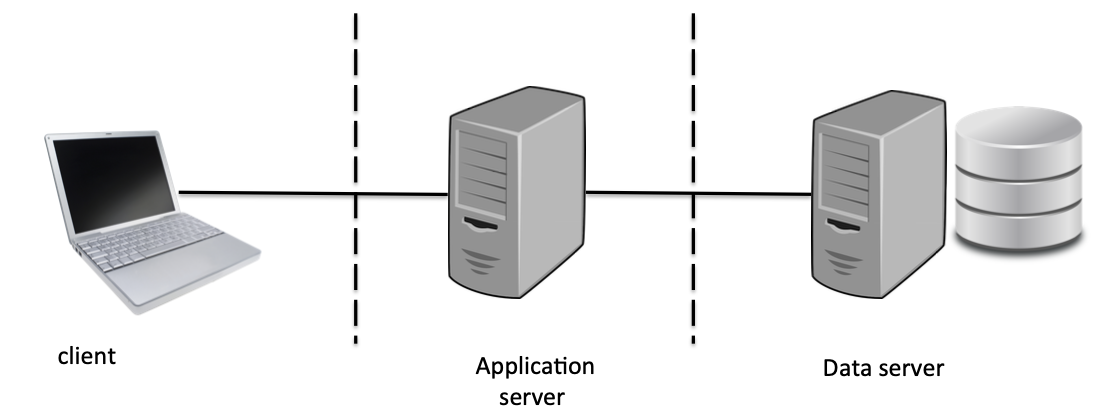
\includegraphics[width=0.7\textwidth]{ThreeTiered}
	\caption{3-Tiered architecture}
	\centering
	\label{fig:ThreeTieredArchitecture}
\end{figure}


\textbf{Tier-1} is the \textbf{Presentation Layer}.
This layer will deploy the Click Client's Mobile Application,
the Store Manager's Management System,
and even Digital Counterpart and Ticket Hand-Out Machine's presentation.

\textbf{Tier-2} is the \textbf{Logic Application Layer}.
This layer will deploy our Back-End System's components.

\textbf{Tier-3} is the \textbf{Data Access Layer}.
This layer includes our DBMS and the Data Base.

Finally, our high-level architecture is shown in Fig.\ref{fig:HighLevelArchitecture}.
The Store Manager's PC and other hardware will connect with the Ethernet Switch Hub.
The Click Customer's Mobile App will communicate with our Back-End System via the Internet.

\begin{figure}[H]
	\centering
	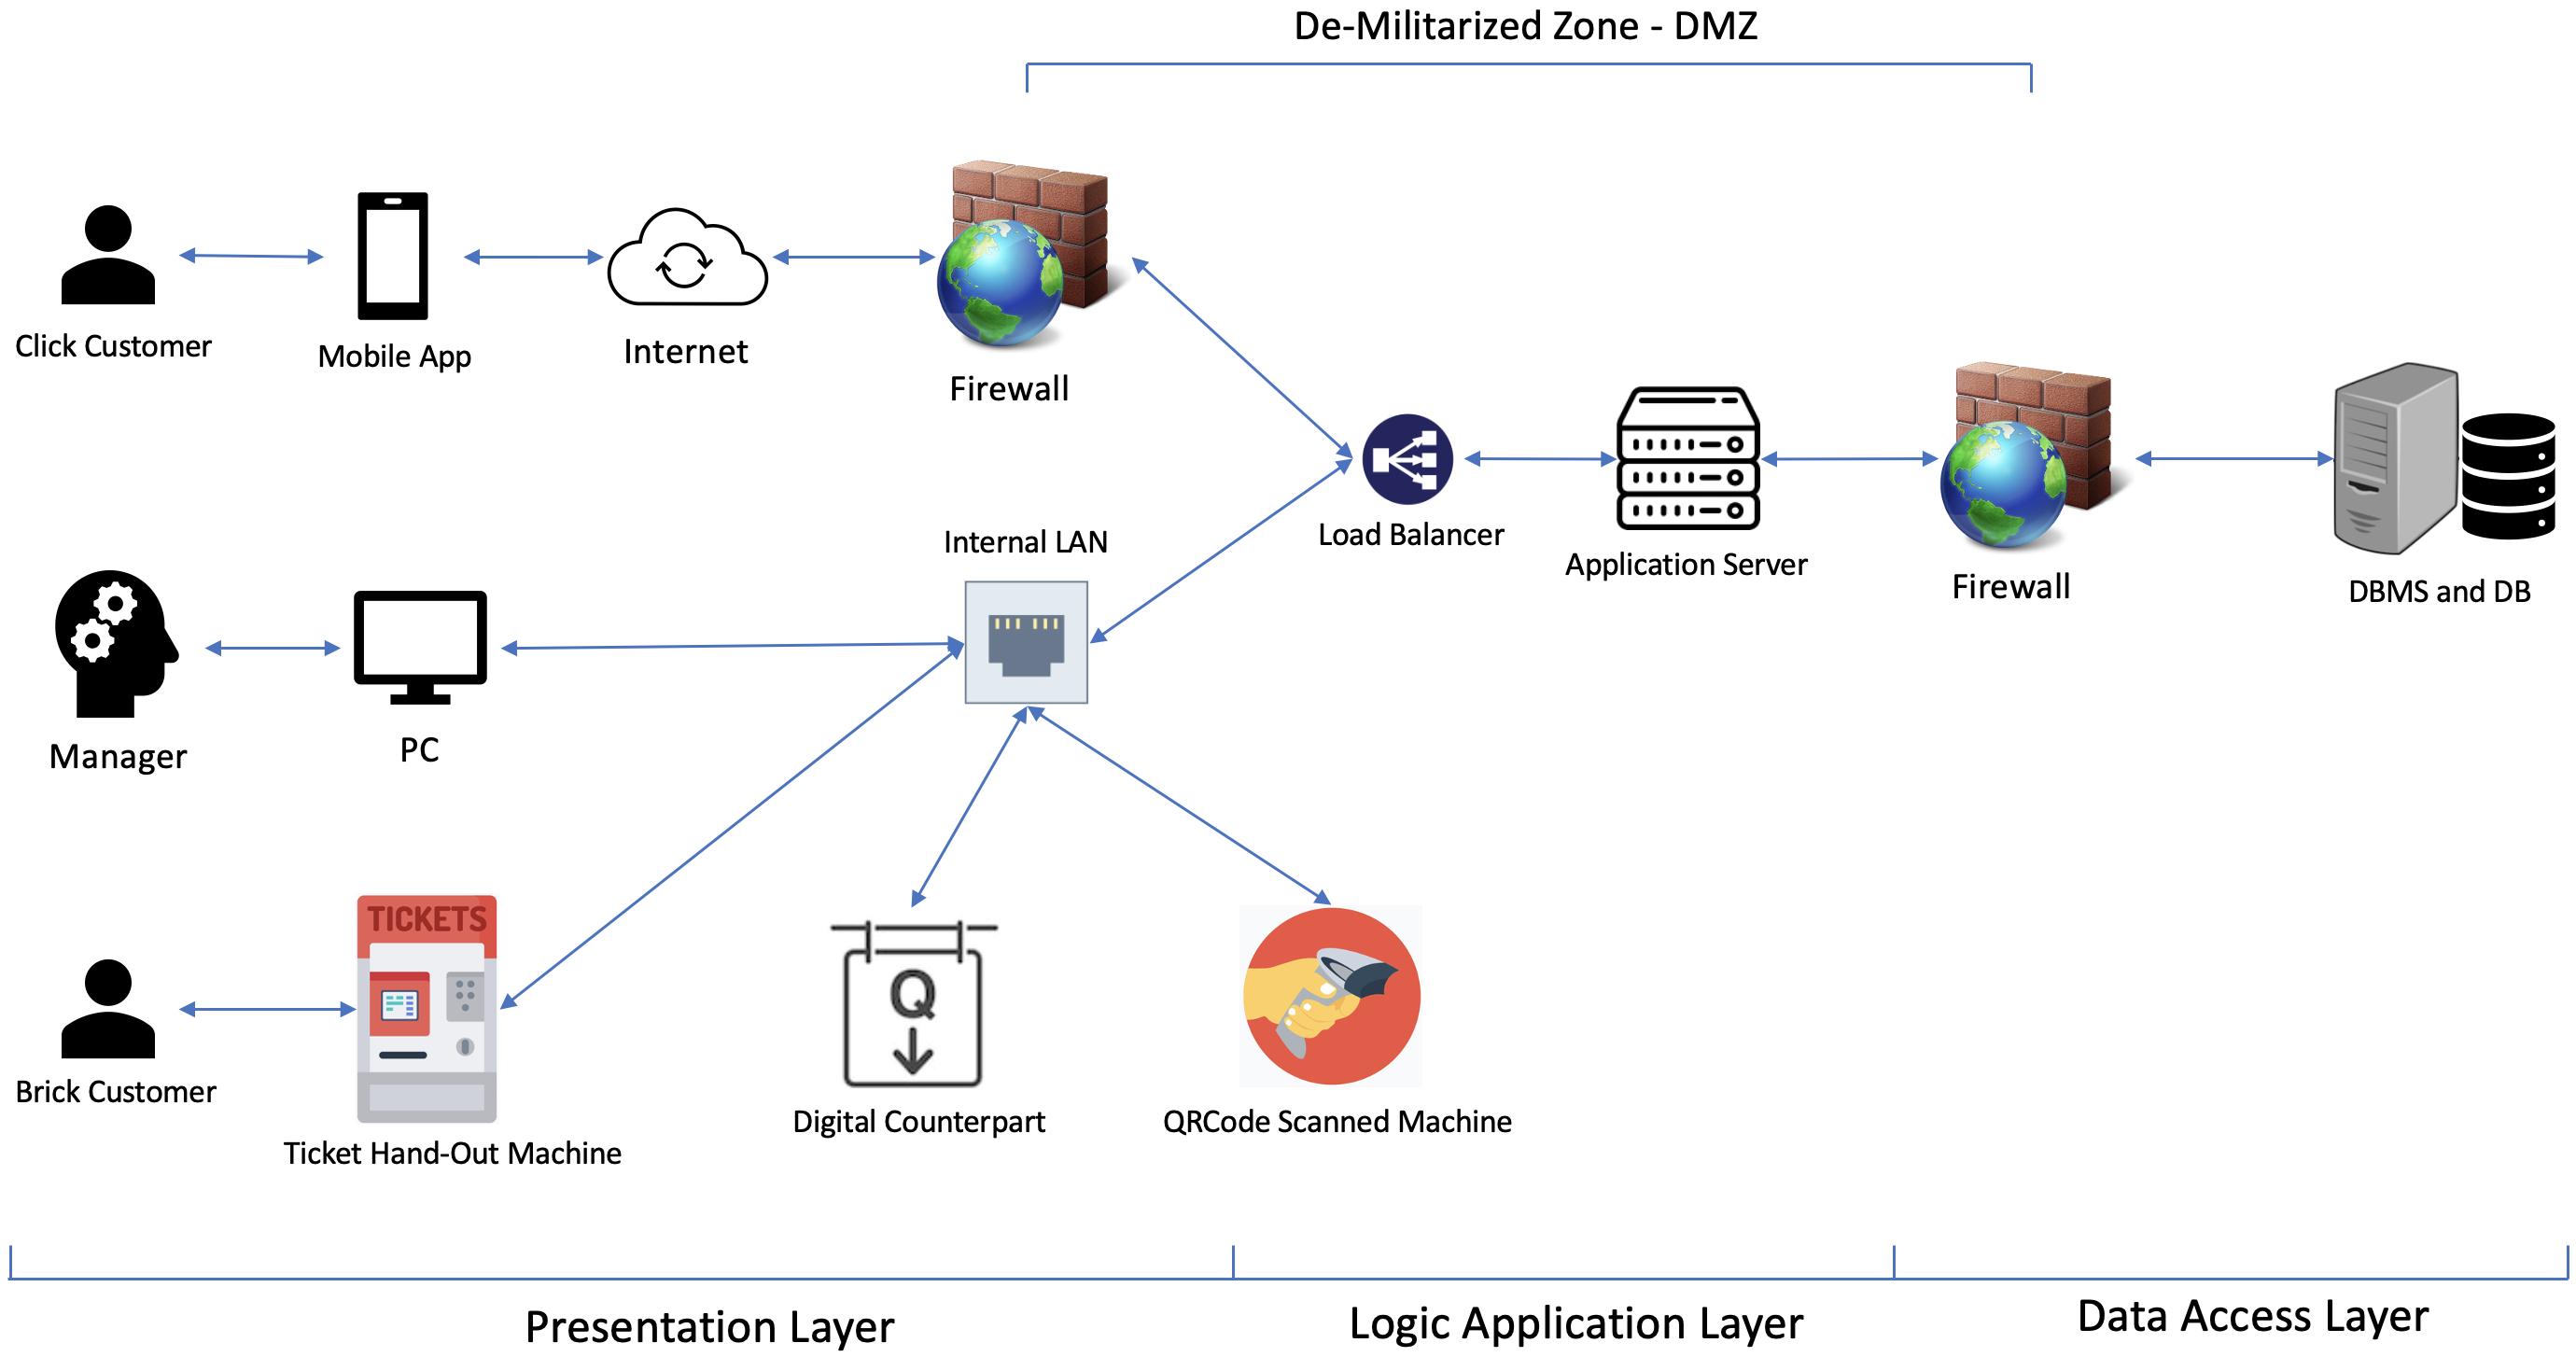
\includegraphics[width=1.2\textwidth]{HighLevelArchitecture}
	\caption{High level architecture}
	\centering
	\label{fig:HighLevelArchitecture}
\end{figure}

More detailed components will be introduced in the next sections.
In particular, in Sec.\ref{sec:deployment-view}.
There, we will introduce the DMZ, load balancer, and other Deployment plan selections.


\section{Component View} \label{sec:ComponentView}
The following diagram Fig.\ref{fig:ComponentDiagram} is the \textbf{Component Diagram}, and it contains all components in our system.
This diagram shows the 3-Tiered Architecture of our system.
The Yellow components are in Presentation Layer.
The blue components are in the Logic Application Layer, and the Green components DBMSServer is in the Data Access Layer.
We will separately introduce all these components in this section, for the interfaces, please go to Sec.\ref{sec:component-interfaces}.

\begin{figure}[H]
	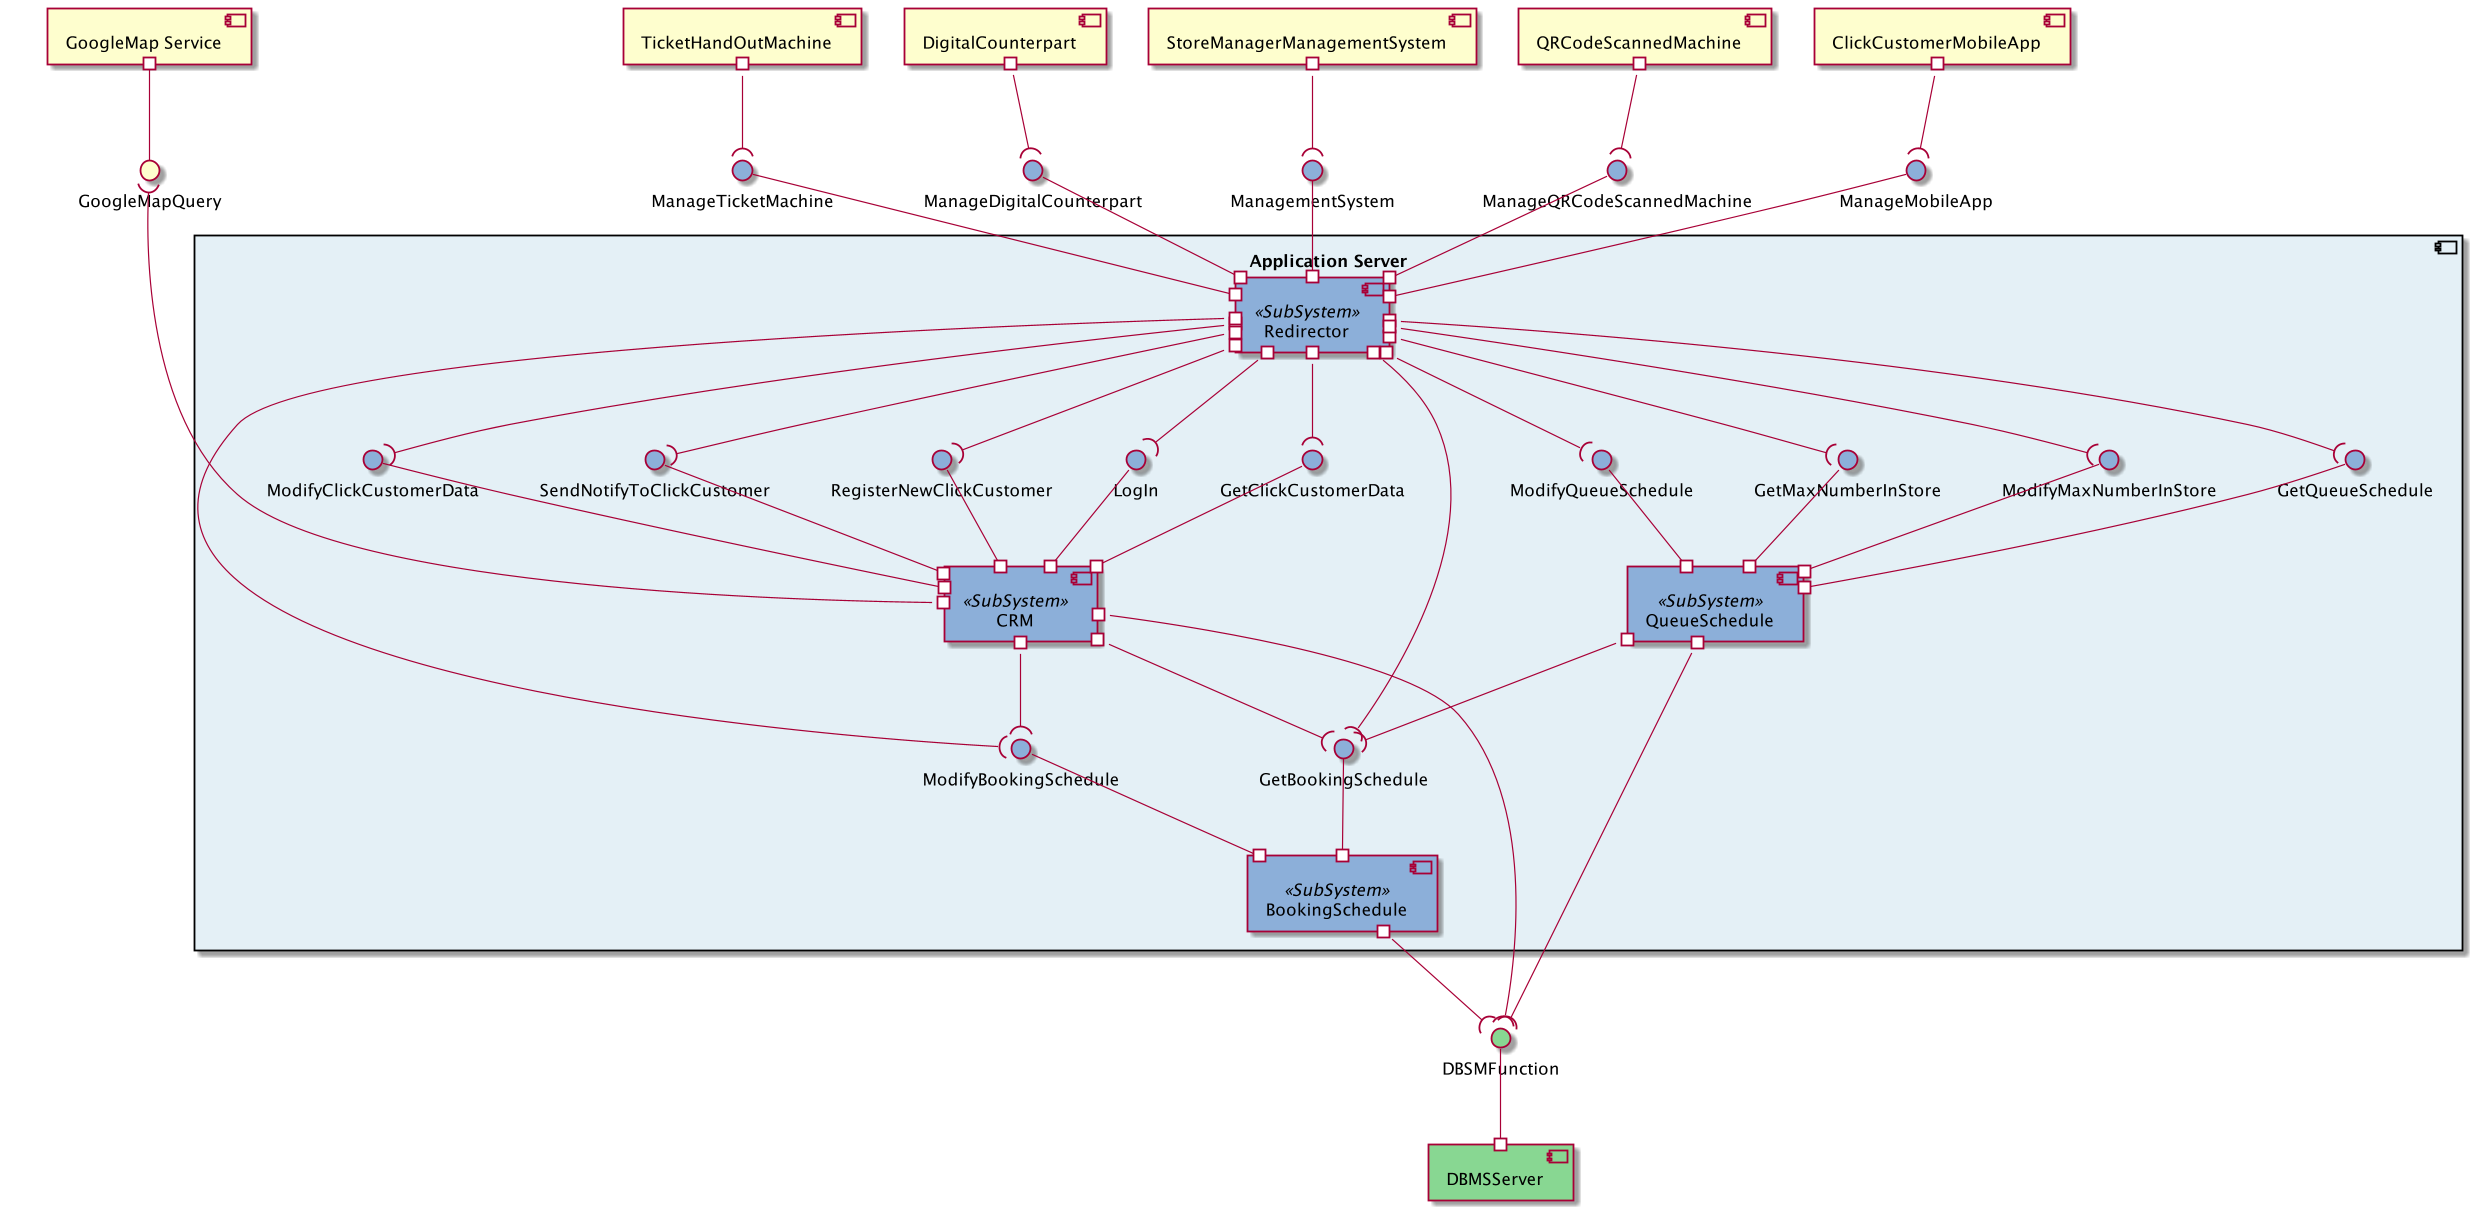
\includegraphics[width=1.2\textwidth]{component_diagram}
	\centering
	\caption{Component Diagram}
	\label{fig:ComponentDiagram}
\end{figure}


The \textbf{Redirector} component is a bridge for communicating the Presentation Layer and the Logic Application Layer.
It is transparent to User and back-end systems, plays the role of forwarding information on both sides, and connect interfaces.
It has four subsystems, respectively, responsible for communicating with four types of devices, as shown in Fig.\ref{fig:component_diagram_redirector}.


\begin{figure}[H]
	\centering
	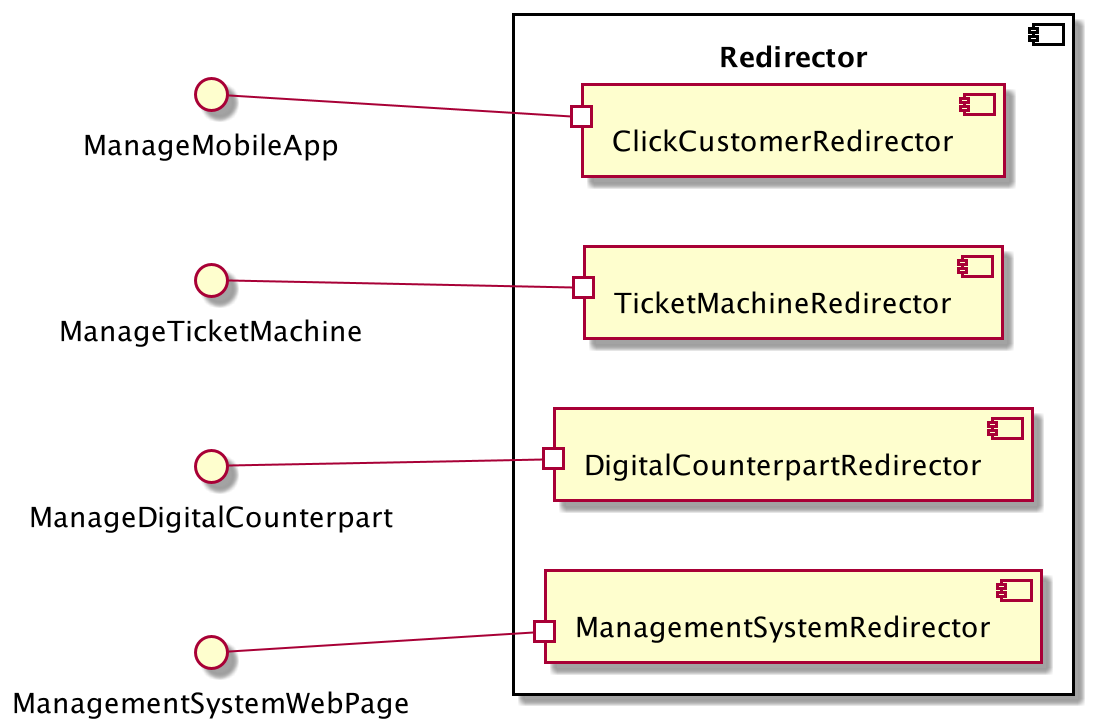
\includegraphics[scale=0.2]{component_diagram_redirector}
	\caption{Redirector Component Diagram}
	\centering
	\label{fig:component_diagram_redirector}
\end{figure}

\begin{figure}
	\centering
	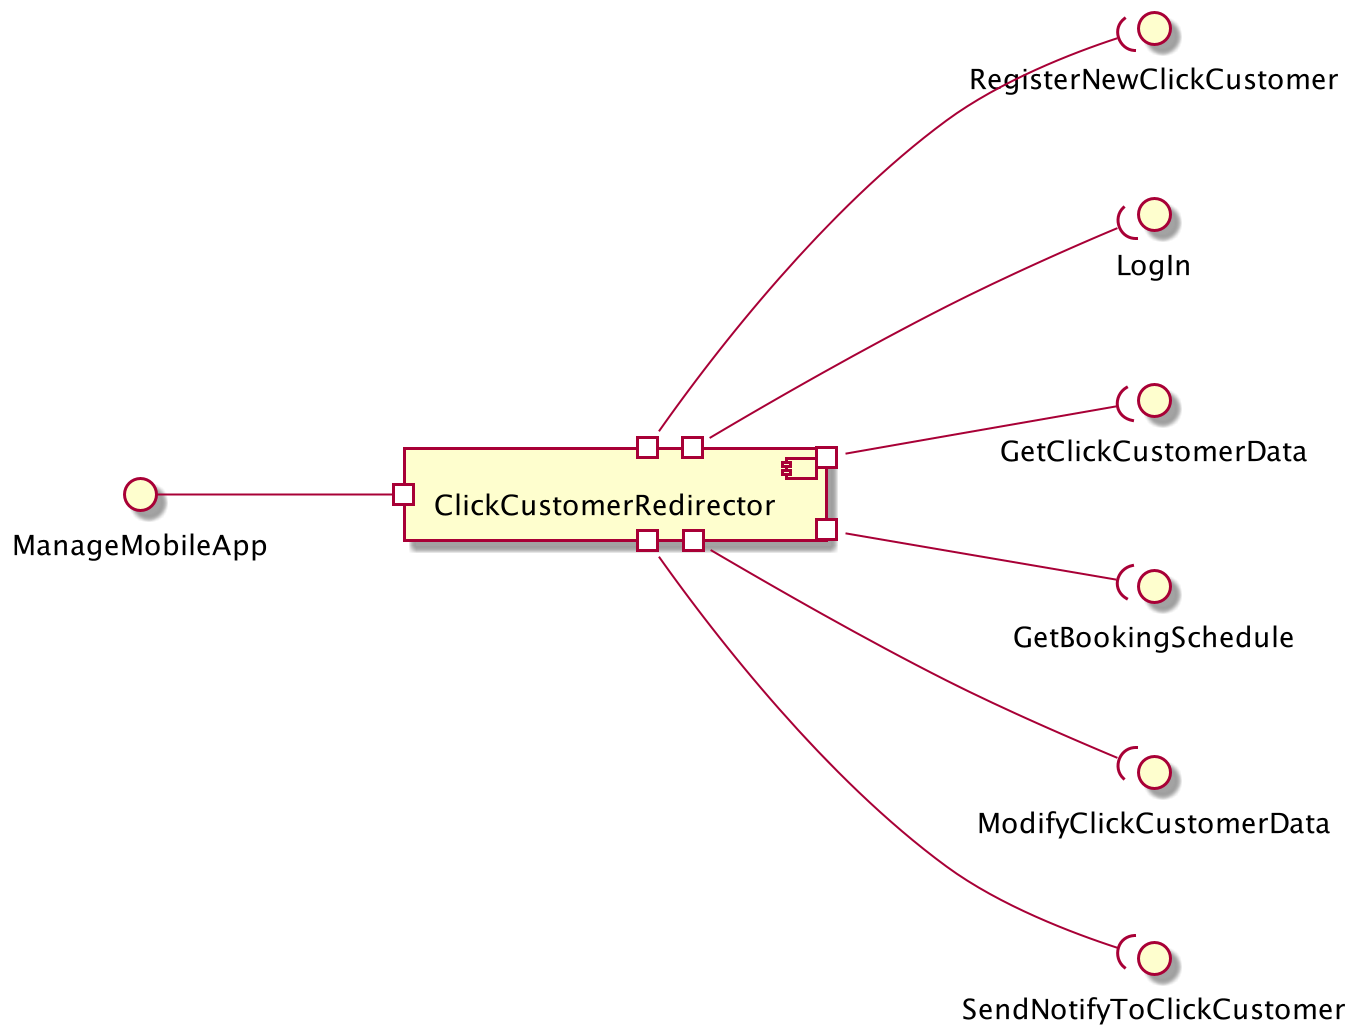
\includegraphics[width=0.8\textwidth]{component_diagram_ClickCustomerRedirector}
	\vspace{10mm}
	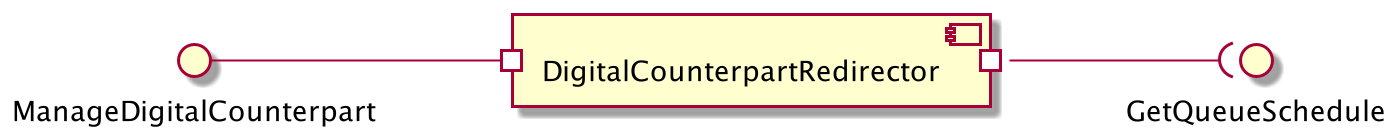
\includegraphics[width=0.8\textwidth]{component_diagram_DigitalCounterpartRedirector}
	\vspace{10mm}
	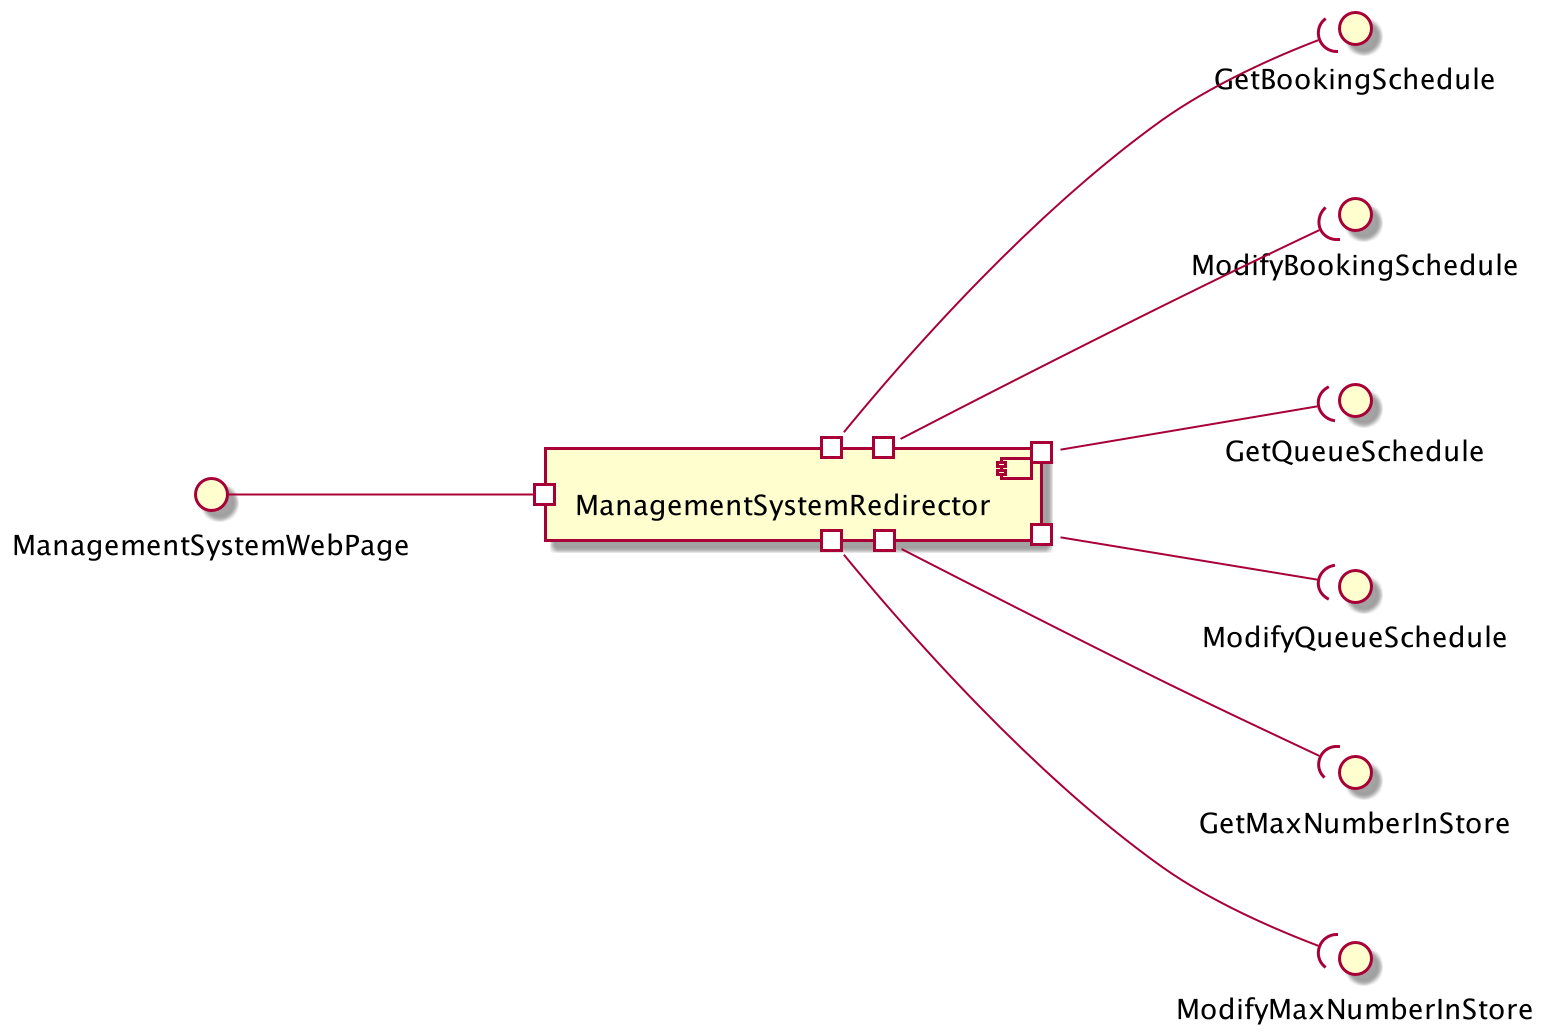
\includegraphics[width=0.8\textwidth]{component_diagram_ManagementSystemRedirector}
	\vspace{10mm}
	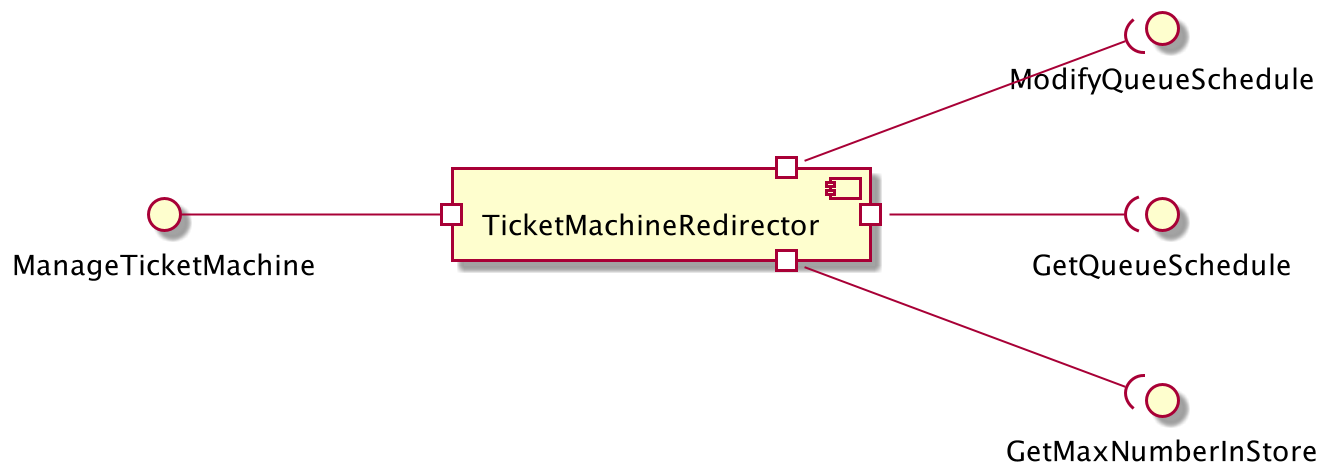
\includegraphics[width=0.8\textwidth]{component_diagram_TicketMachineRedirector}
	\vspace{10mm}
	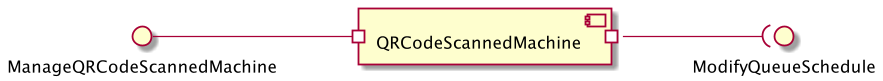
\includegraphics[width=0.8\textwidth]{component_diagram_QRMachine}
	\vspace{10mm}
	\caption{Redirector's Subsystem Component Diagram}
	\centering
	\label{fig:component_diagram_RedirectoSubsystem}
\end{figure}



The \textbf{ClickCustomerRedirector} will transfer the message between Mobile Application and the Application Server.
The Register message will pass by the RegisterNewClickCustomer, and look out the Valid/History Booking will use the GetClickCustomerData Interface,
this Interface will return all information of this Customer.
For the most important operation - Booking a visit, use GetClickCustomerData to get the available Time/Date and the average history duration(if available).
Then, through the ModifyClickCustomerData Interface to submit the Booking,
by the way, it also can modify other available data of this Customer.
Moreover, the SendNotifyToClickCustomer Interface will handle Notify message.
The Mobile Application can actively "pull" Notify message through this Interface from the Back-End System.
To "push" Notify information, we will use the Observer Pattern.
It will introduce in Sec.\ref{sec:SelectedArchitecturalStylesAndPatterns}

The \textbf{TicketMachineRedirector} will transfer the Ticket Hand-Out Machine's message.
It needs two pieces of information, the allowed \hyperref[subsec:definitions]{maximum number of people in the store} and how many Customers in the Queue in time.
So The GetQueueSchedule and GetMaxNumberInStore Interface can do these operations, and these two fields will show on the Ticket Machine's screen.
Finally, the retrieve ticket operation will handle by the ModifyQueueSchedule Interface.
It will put a BrickCustomer into the Queue.

The \textbf{DigitalCounterpartRedirector} will help the \hyperref[subsec:definitions]{Digital Counterpart} display the next queue number.
The Customer can enter the store after found his number on the Digital Counterpart.

The \textbf{ManagementSystemRedirector} will function for the Management System of our Store Manager.
This redirector will transmit the message between the Presentation layer's web page and the Back-End System.
Through the Interface shown in Fig.\ref{fig:component_diagram_RedirectoSubsystem}, the Manager can realize his operation like reschedule someone's Booking, adjust the Queue order, or lower the maximum number.

The \textbf{QRCodeScannedMachineRedirector} is working for the \hyperref[subsec:definitions]{Ticket QRCode Scanned Machine}.
When the Enter Machine scanned someone's QRCode, it will directly use the ModifyQueueSchedule to move this Customer from the Queue list to the CustomerInStore list.
If this Customer is not in the Queue list, the ModifyQueueSchedule will not return OK, which means this operation not successful.
Of course, the Exit Machine will do similar things, move out the Customer from the CustomerInStore list.


The next three subsystems are the core subsystems in our application layer.

The \textbf{CRM} component is responsible for communicating with Click Customers' End, handle the register, Log-In, Booking, data-send, and notify-send operation.
The Booking operation will communicate with the Booking Schedule component, get the available data/time, send the Booking Information, generate E-Ticket, and store all data in the database.
In addition, it must also help the Customer calculate the estimated departure time from depart place to the store, so it will call the GoogleMap API to query it.

The \textbf{Booking Schedule} component is working for all Booking tasks.
Receive the Booking from CRM, handle the Store Manager's modified Booking, send the Booking schedule to the Queue Schedule component, and store all Booking Schedule to the database.

The \textbf{Queue Schedule} subsystem is the main component to communicate with the Store Manager's Management System.
It has to take the Booking schedule to calculate the Queue order and handle the Store Manager's modification for the Maximum value or Queue order.

At last, the \textbf{Database System}, it will manage all database, and handle the CRM, BookingSchedule, QueueSchedule's Query/Insert/Update.




\newpage
\section{Deployment View}\label{sec:deployment-view}

Our deployment situation, as shown in Fig.\ref{fig:deployment_diagram}.
Three colors respectively represent the three layers.
The Green devices are in the Data Access Layer, the Blue devices are in the Logic Application Layer,
and the Yellow devices are in the Presentation Layer.

\begin{figure}[H]
	\centering
	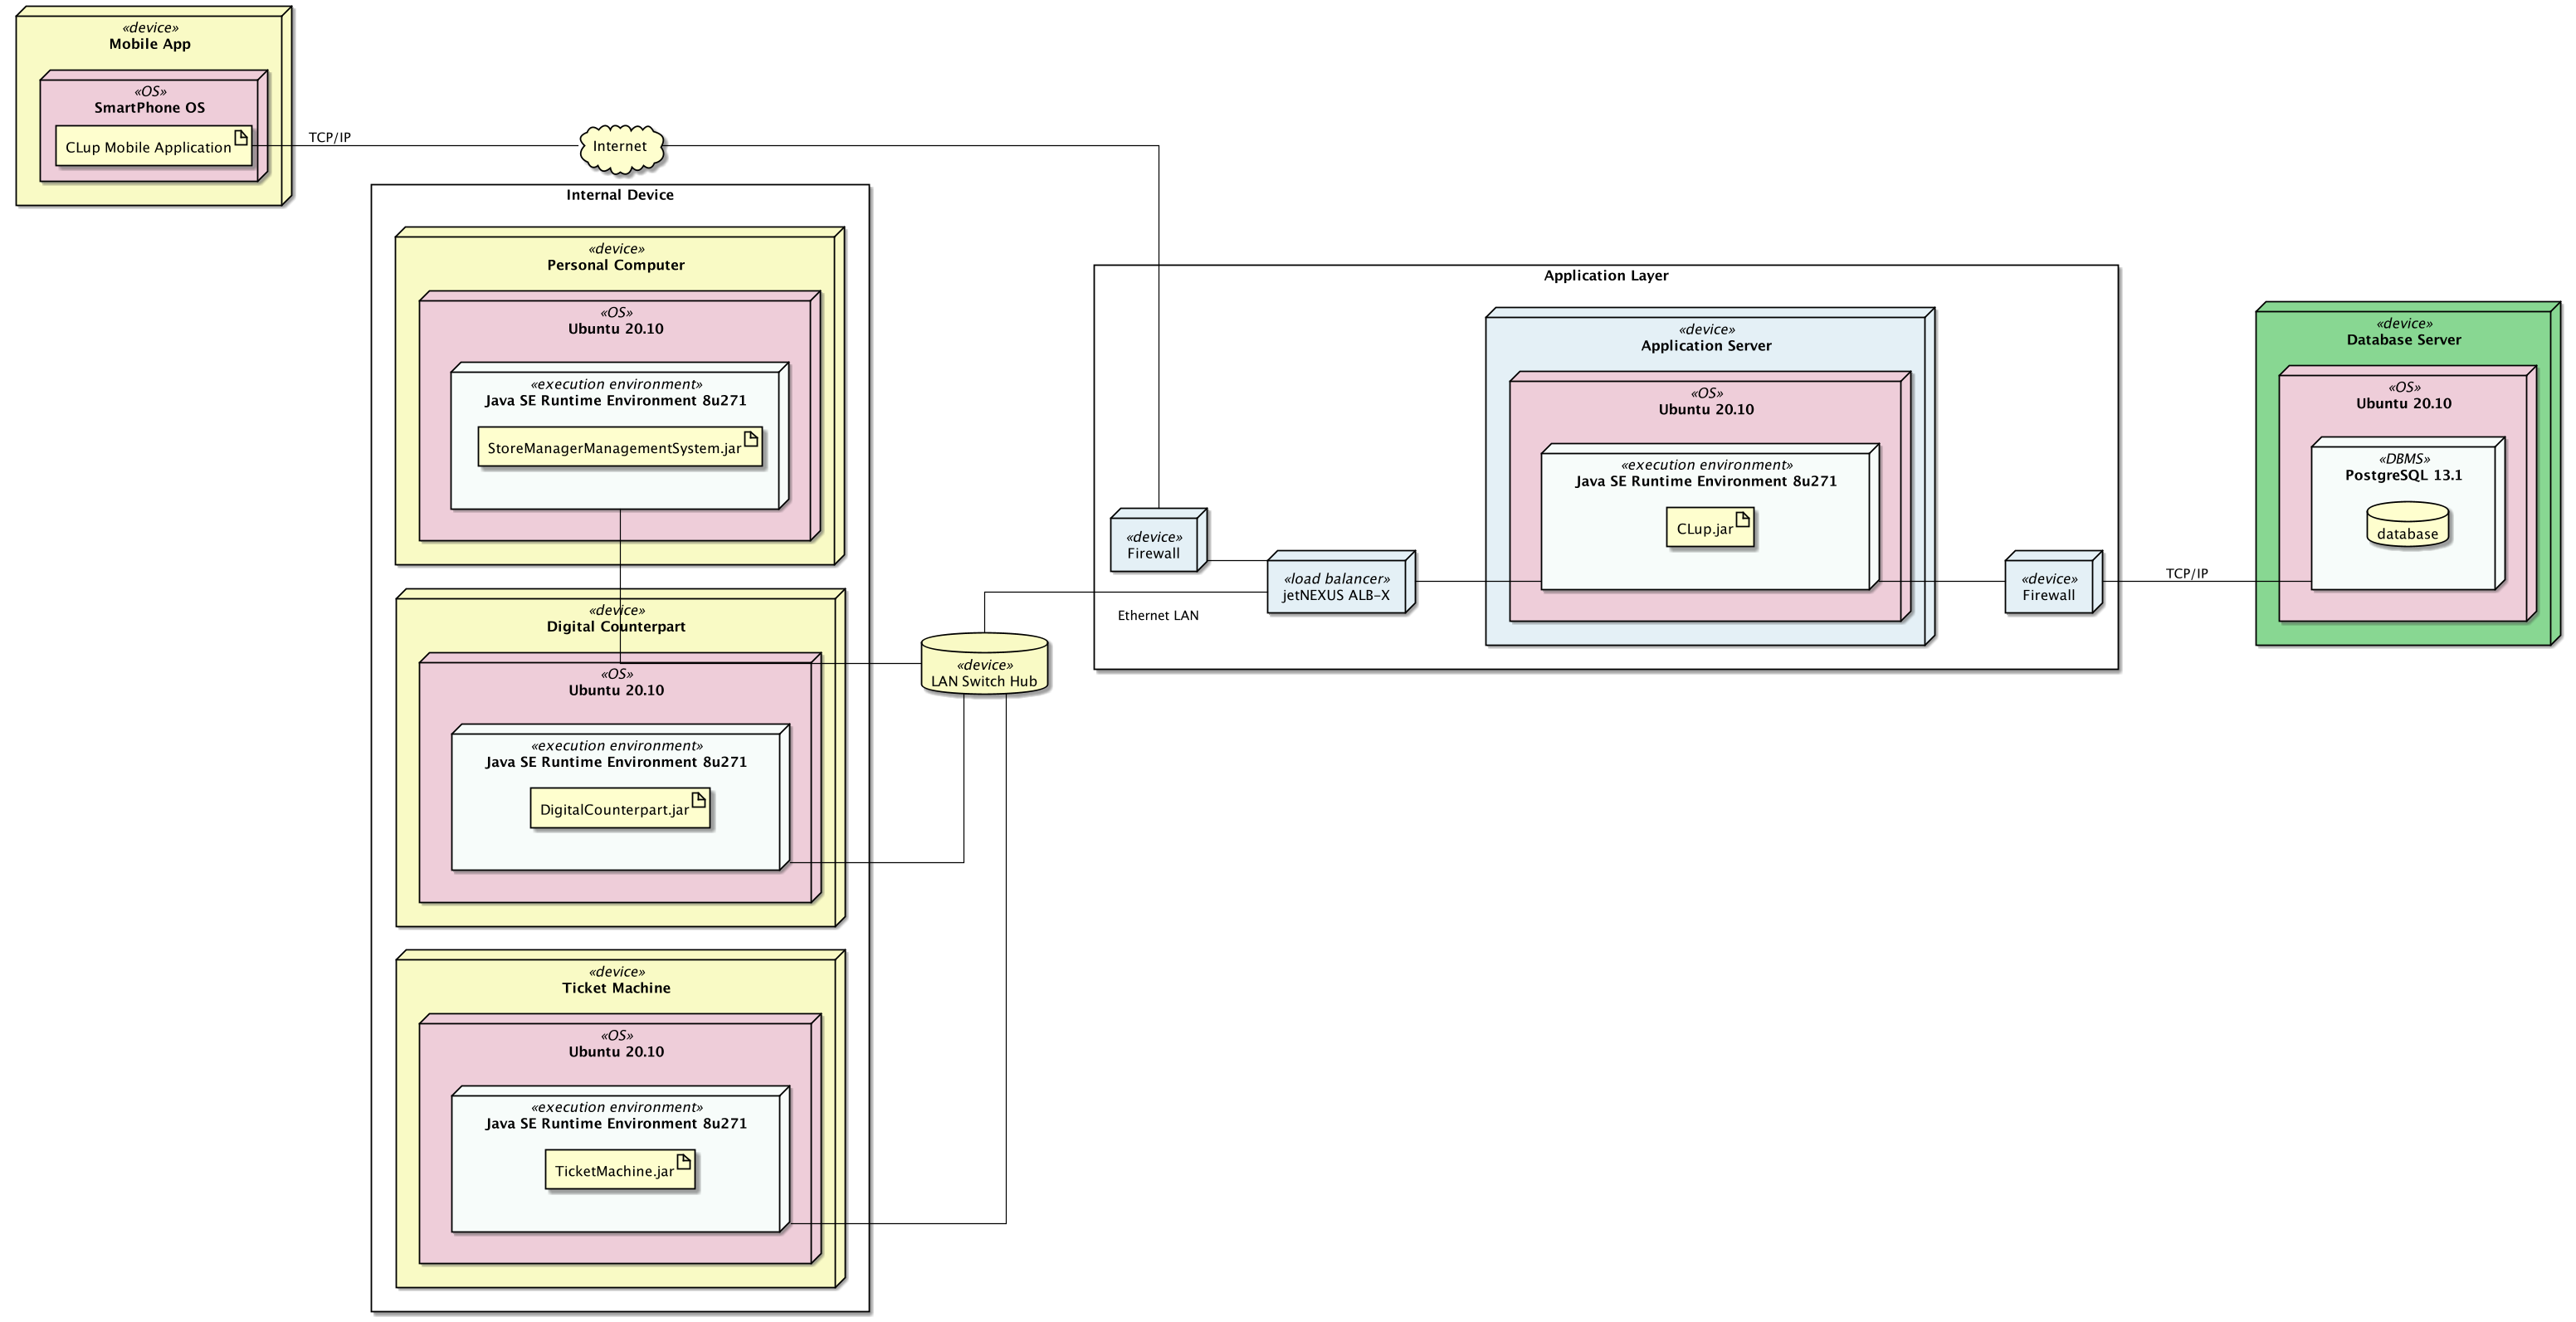
\includegraphics[width=1.2\textwidth]{deployment_diagram}
	\caption{Deployment Diagram}
	\centering
	\label{fig:deployment_diagram}
\end{figure}

For all our devices, to reduce the development/management/maintenance cost,
we will use the same Operation System - Ubuntu 20.10, and run in the same Runtime Environment - Java SE Runtime Environment 8u271.

In the \textbf{Presentation Layer}, The Store Manager's PC, the Digital Counterpart, the Ticket Machine and the QRCode Scanned Machine are the Internal Devices, which means we must manage them by ourselves.
We built a LAN to connecting them with the Application Server via the Switch Hub.
In our LAN, we used the Ethernet Protocol.
Moreover, we have chosen the \textbf{Thin Client} strategy in the system architecture, so all our Internal Devices can run on the Raspberry Pi 4.
It is a very low-cost deployment solution.

In contrast, the Mobile Application is the External Device that will run on the Click Customer's SmartPhone.
It has to connect with Back-End System via the Internet.
We will separately develop the Client End for the two kinds of systems - IOS and Andriod System.

In the \textbf{Application Layer}, We refer to the network security part of the information system book P.243.
We used two Firewalls to build a \textbf{DeMilitarized Zone - DMZ}.
The external network can only access the resources exposed in the DMZ (Our Application API), and the rest of the network is behind the second firewall.
The DMZ functions as an isolated subnet between the Internet and the private network,
So that our database can be better protected.\cite{SistemiInformativi}

For the \textbf{Load Balancer}, we must first ensure that our Internal Devices can allocate enough Server resources and then ensure the Click Customer's resources, so we considered two plans.
\begin{enumerate}
	\item Allocate dedicated Application Servers for our Internal Device, and other Application Servers connect with Load Balancer.
	\item Do not allocate server resources separately for internal devices, but set higher weights for Internal Devices in the load balancer.
\end{enumerate}
Plan 1 can guarantee that our system's most important part can work well, whether the balancer is working or how crowded the network is.
Plan 2 ensures that when some servers are not working, the well-function servers can always allocate to Internal Devices.
After weighing, we finally chose plan 2.
Because we think Plan 2 has higher system availability/maintainability.

As mentioned above, for the \textbf{Application Server}, we adopted the Reliable Array of Cloned Services - RACS, like the figure in the Information System Book P.202\cite{SistemiInformativi}, Fig.\ref{fig:RACS}.
The load balancer must allocate the higher weights to Internal Devices, and all our Application Server will run the same application.
There is a different point in our case from the figure: we have separated the database and the Application Server.
Nevertheless, cause our business is "write-intensive", so we used the shared-disk configuration in essence.

\begin{figure}[H]
	\centering
	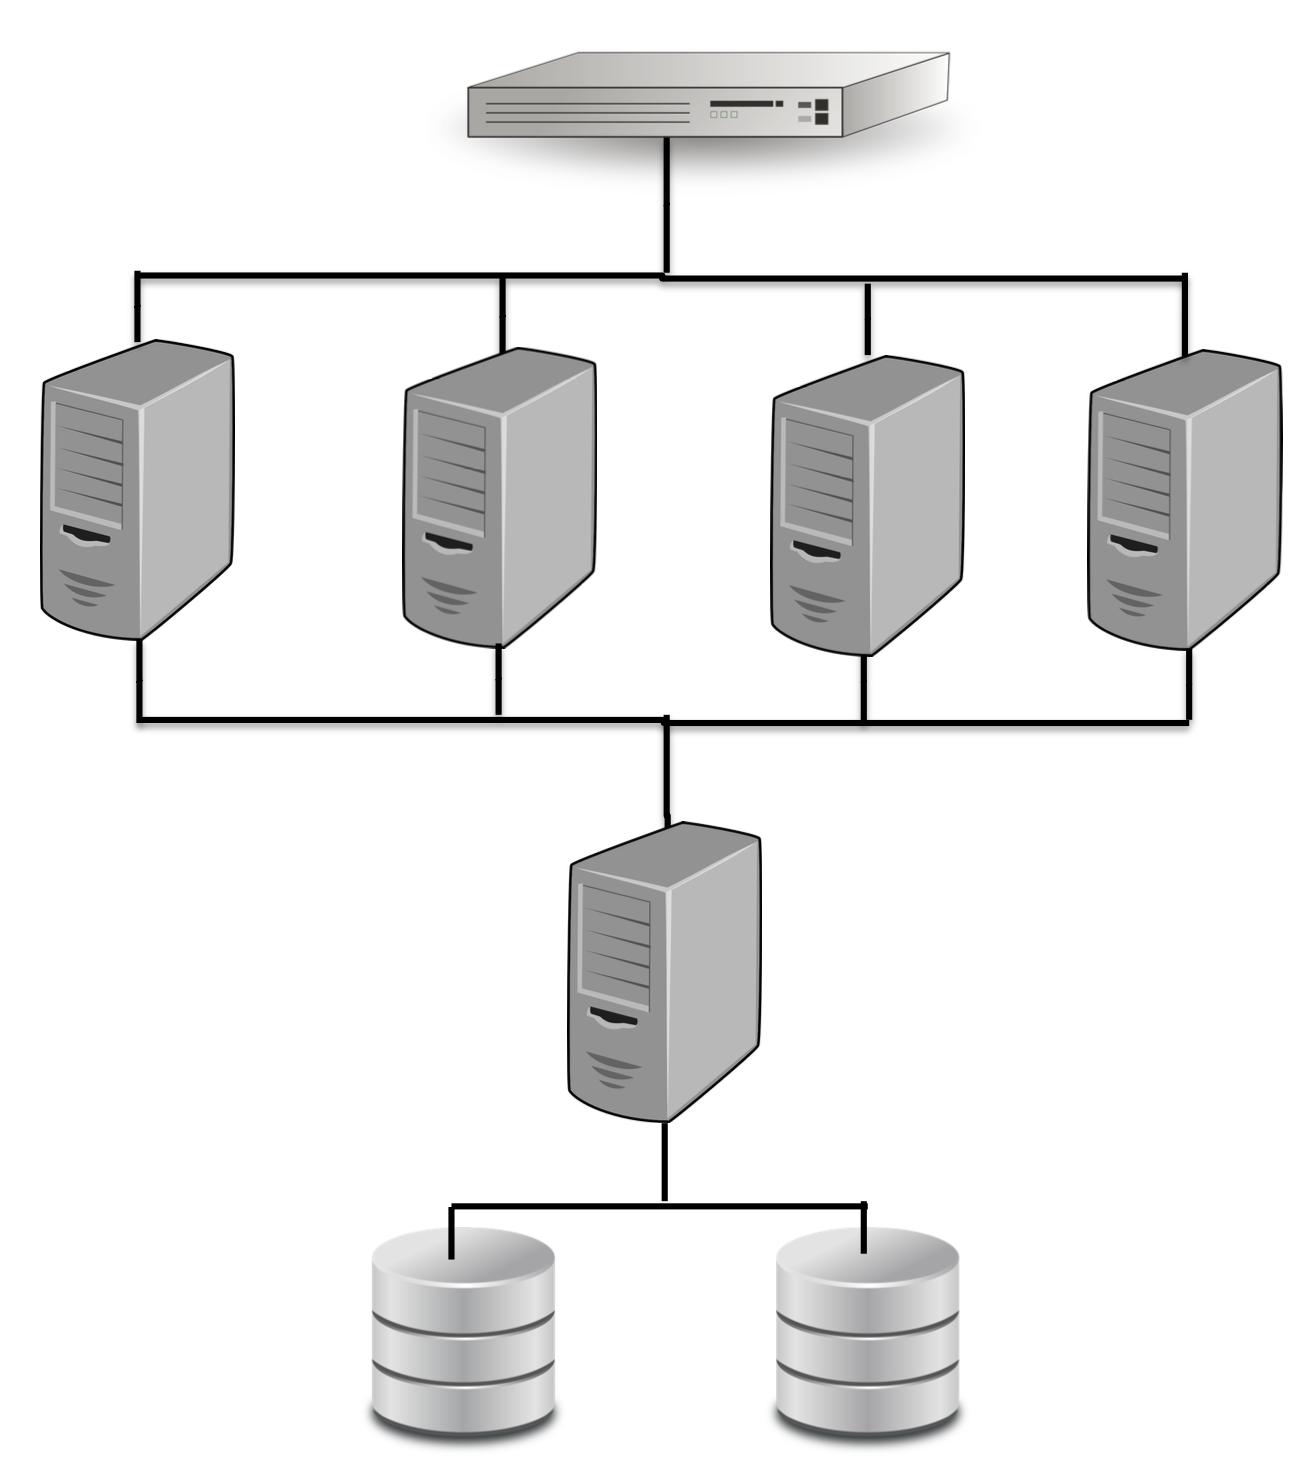
\includegraphics[width=0.4\textwidth]{RACS}
	\caption{RACS: Shared-disk o cluster Configuration}
	\centering
	\label{fig:RACS}
\end{figure}


Finally, the \textbf{Database system}, we selected PostgreSQL as the Database Management System cause it is Open Sources and stable.
Then we will use the relational database to implement it.
For Security, as the DMZ mentioned above, only our private network can access this system, so that the external network will difficultly attack our database.


\section{Runtime View}\label{sec:RuntimeViwe}

This section will describe the two most important processes in our system - the Click Customer booking process and Store Manager manage processes.

The \textbf{Click Customer booking process} is shown in Fig.\ref{fig:ClickCustomerBookingFunction}.
There are three components of our Application Server participated in.
The redirector forward all message for two sides, and the CRM system handle all Customer stuffs like the bank windows.
When a Customer sends a booking, the CRM system will not generate tickets immediately.
Because it must wait for all customers within the closed period to book their visit, and then it can calculate the route map in the Store for each customer according to their wanted list.
By the way, there we used the Observer Pattern, which we will introduce in Sec.\ref{sec:SelectedArchitecturalStylesAndPatterns}.
However, the CRM will generate the Ticket when someone's booking is changed and then send a notification to the corresponding Customer.

After-all, the Customer can check their Ticket when they received the Notification.
If they checked it too early, they would only found their historic Ticket.


The second process is the \textbf{Store Manager Management System process}, and it is shown in Fig.\ref{fig:StoreManagerManagementSystemSequenceDiagram}.
This process presented all functions of the Store Manager Management System.
The four operations in the figure are independent of each other, and there is no sequence.
The management system can execute any process according to the operations of the Store Manager.
Since the first three operations in the figure are clear and precise enough, we will focus on the fourth operation - Reschedule the booking.

When a Store Manager does the \textbf{Rescheduling job}, they have to check the Booking Schedule first, and then choose a range they want to change,
for example, the Click Customers who want to visit the Gelato area.
And then, submit the change through the ModifyBookingSchedule API.
The BookingSchedule component will store this change in the database.
At this time, our Observer Pattern will function, the CRM will find out this change and regenerate the Ticket for the corresponding Click Customer if it is needed.
Cause it is not a part of the Management System, so not shown in this Figure.

\begin{figure}[H]
	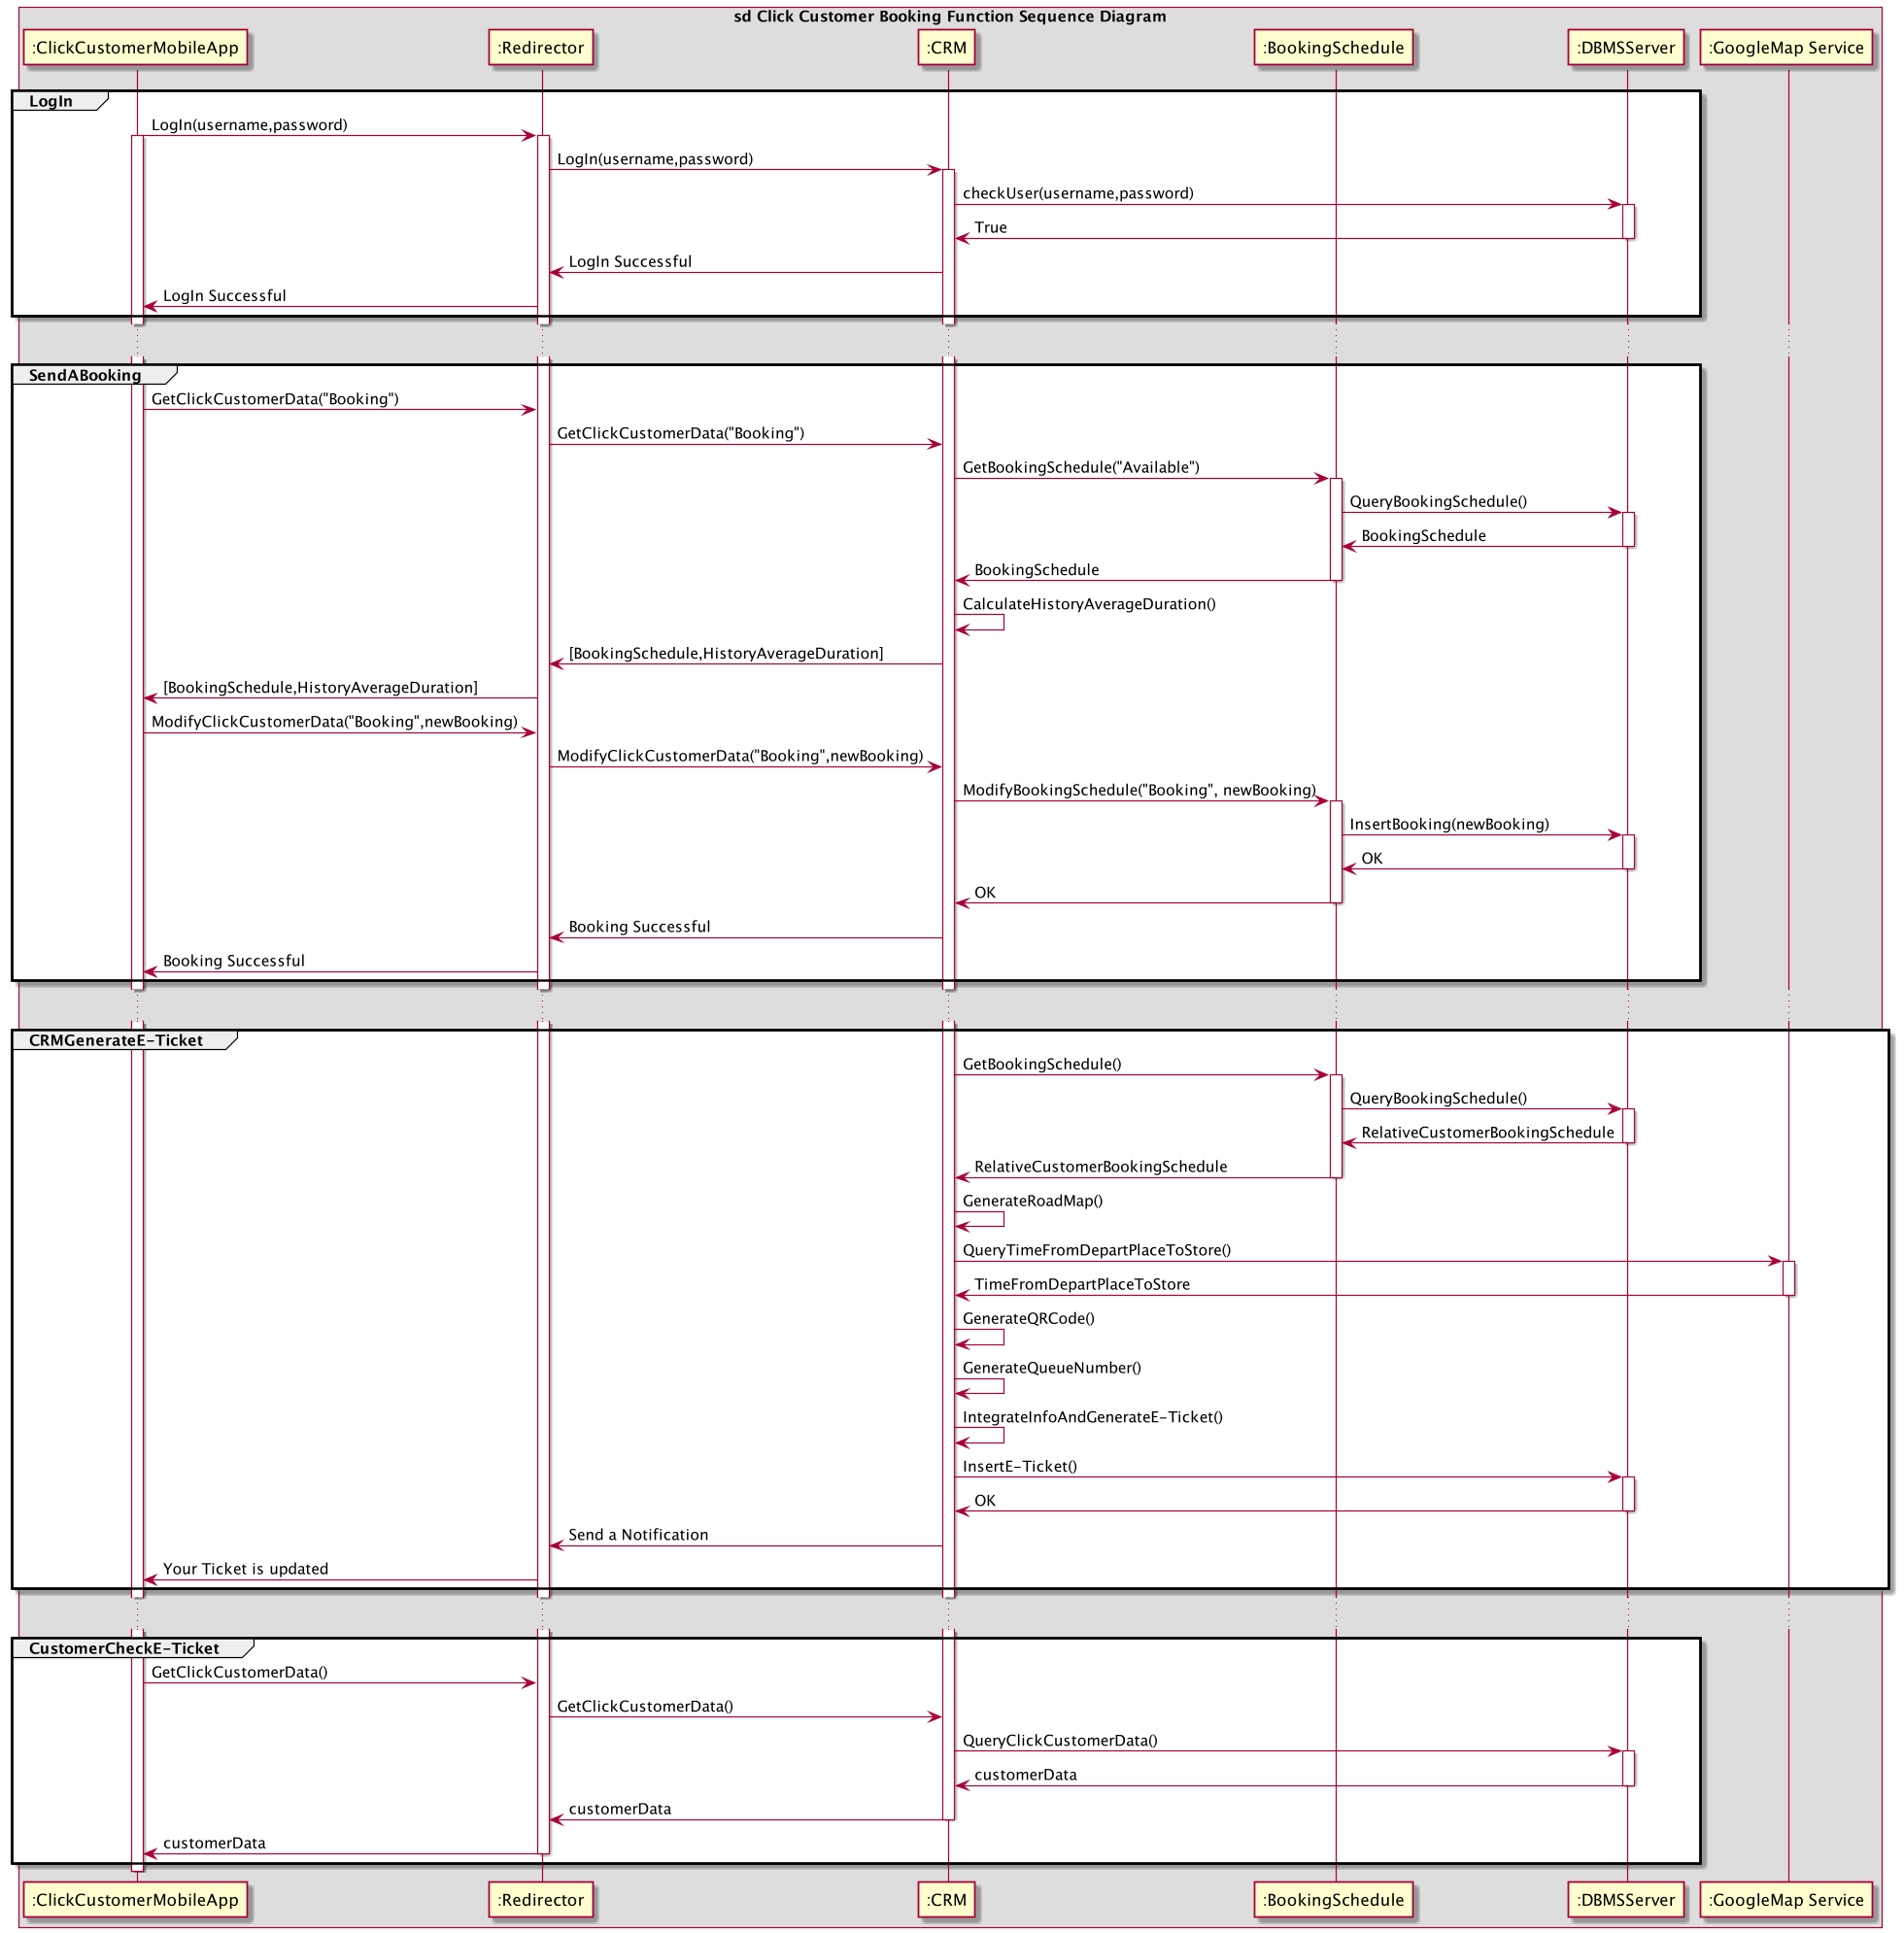
\includegraphics[width=1.2\textwidth]{sequence_diagram_ClickCustomerBookingFunction}
	\centering
	\caption{Click Customer's Booking Function Sequence Diagram}
	\label{fig:ClickCustomerBookingFunction}
\end{figure}

\begin{figure}[H]
	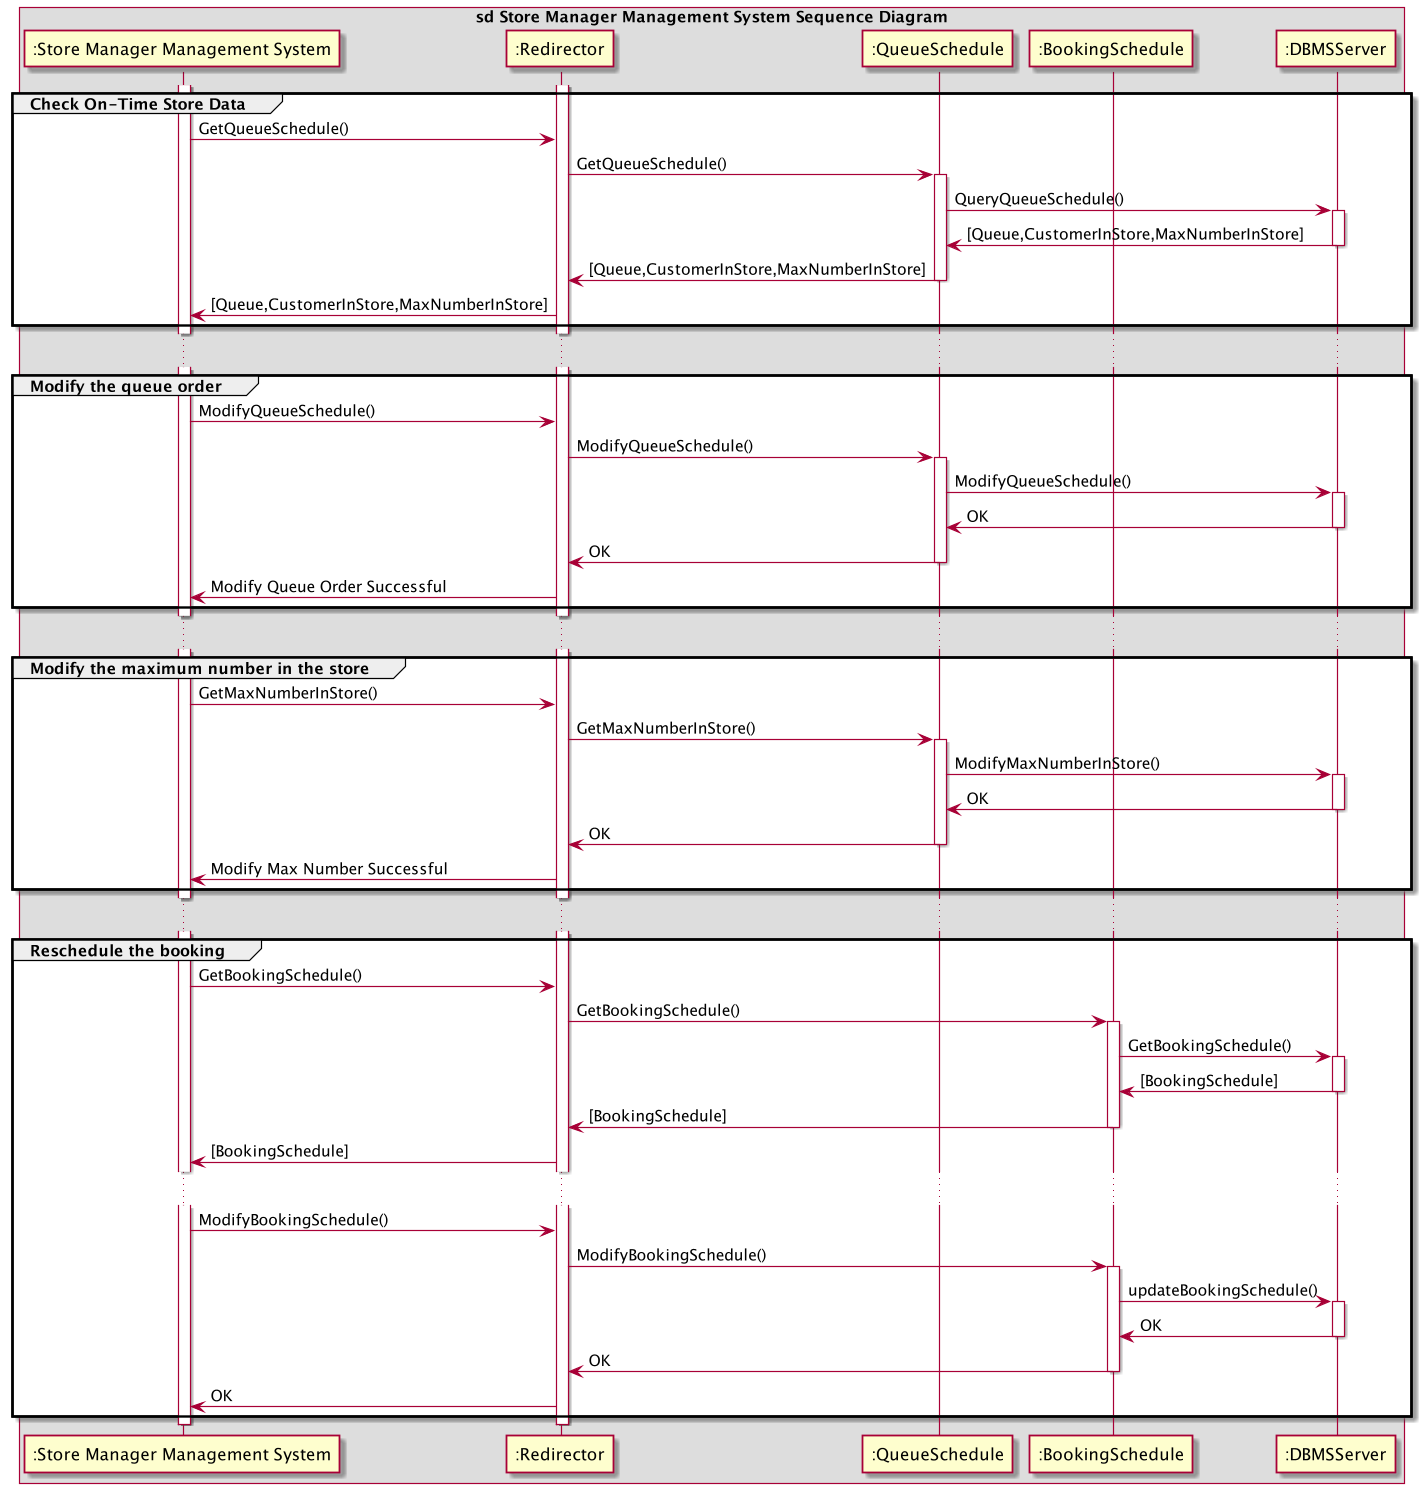
\includegraphics[width=1.2\textwidth]{sequence_diagram_StoreManagerManagementSystem}
	\centering
	\caption{Store Manager Management System Sequence Diagram}
	\label{fig:StoreManagerManagementSystemSequenceDiagram}
\end{figure}


\section{Component Interfaces}\label{sec:component-interfaces}

The fundamental relationship between Interface and components has been illustrated in the component diagram Fig.\ref{fig:ComponentDiagram}.
So, in this section, we will introduce each Interface in detail.

\vspace{5mm}

For \textbf{CRM}'s Interface:
\begin{itemize}
	\item RegisterNewClickCustomer(username, password): It is only for the Click Customer Mobile App to register the new User.
	\item LogIn(username,password): It is for registed user log-in.
	\item GetClickCustomerData(motive): It can get all Current/History Ticket.
	If the motive value is "Booking", it can also get the Historic Average duration and the available booking date/time for the Booking operation.
	\item ModifyClickCustomerData(): The Mobile App must use this function to contain the new Booking field and send the Booking.
	If the Booking is Successful, it can get the OK string, so that this Booking is already stored in the database, and the Click Customer just waits for the notification.
	\item SendNotifyToClickCustomer(): This function is used to receive notification from the server passively.
	For example, when the Ticket is generated or updated, the Mobile App will get the notification, and the Customer can check the new Ticket.
\end{itemize}

\vspace{5mm}

For \textbf{BookingSchedule}'s Interface:
\begin{itemize}
	\item GetBookingSchedule(datetime, customer, item): It can use to get the wanted BookingSchedule.
			The range is datetime, customer, or item.
			All of these parameters are a list, a datetime range, customer list, or item list;
			this function will return the wanted Booking.
			For example, when the CRM component wants all the available dates/times in the schedule, it can give the current DateTime to this function.
			It will return all schedules from now, so the CRM can calculate and give the available date/time to the Mobile App.
			Alternatively, if the Store Manager Management System wants to get the Customer list who must visit Gelato and Pizza area, it can give the [Gelato, Pizza] to the item field. For sure, it will return all corresponding customers.
	\item ModifyBookingSchedule(): It used for the Management System, or CRM system want to insert or update some Booking, if the database accepted
			the change, it will return the OK string.
\end{itemize}

\vspace{5mm}

For \textbf{QueueSchedule}'s Interface:

\begin{itemize}
	\item GetQueueSchedule(): It can return the Current Queue order, both the Queue and CustomerInStore.
	All our Presentation Layer's device will use it except the Mobile App and the QRCode Scanned Machine.
	The Digital Counterpart will use it to display the next queue number.
	The Ticket Machine will use it to display how many Customers in queue and store, the Management System will use it to check the \hyperref[subsec:definitions]{Store In-Time Data}.
	\item ModifyQueueSchedule(): Management System and Ticket Machine will use it to modify or insert the Queue order.
	Like the ModifyBookingSchedule, only if the database finally accepted this change, it will return the OK string.
	\item GetMaxNumberInStore(): the Ticket Machine will display the Allowed Maximum number in the Store to remind the Customer, and the Management System will also call it to display this value.
	\item ModifyMaxNumberInStore(): The Management System will use this to change the Allowed Maximum number in the Store value to reduce/raise its current customer number.
\end{itemize}


\section{Selected Architectural Styles and Patterns}\label{sec:SelectedArchitecturalStylesAndPatterns}

As the Sec.\ref{sec:ArchitectureOverview} said, we adopted the \textbf{3-Tiered Architecture} style for our system, as Fig.\ref{fig:Classification Of 3-Tier Architecture} in Sistem Information Book P.197 \cite{SistemiInformativi} showed.
There are 13 kinds of 3-Tier architecture configuration.
From Config 1 to 5 are Think Client and 6 to 13 are Thin Client, we decided to use the \textbf{Thin Client} like the Config 7.
So that our Presentation Layer devices can applicate the lowest cost hardware, in this situation, we chose the Raspberry Pi 4 for all these devices.


\begin{figure}[H]
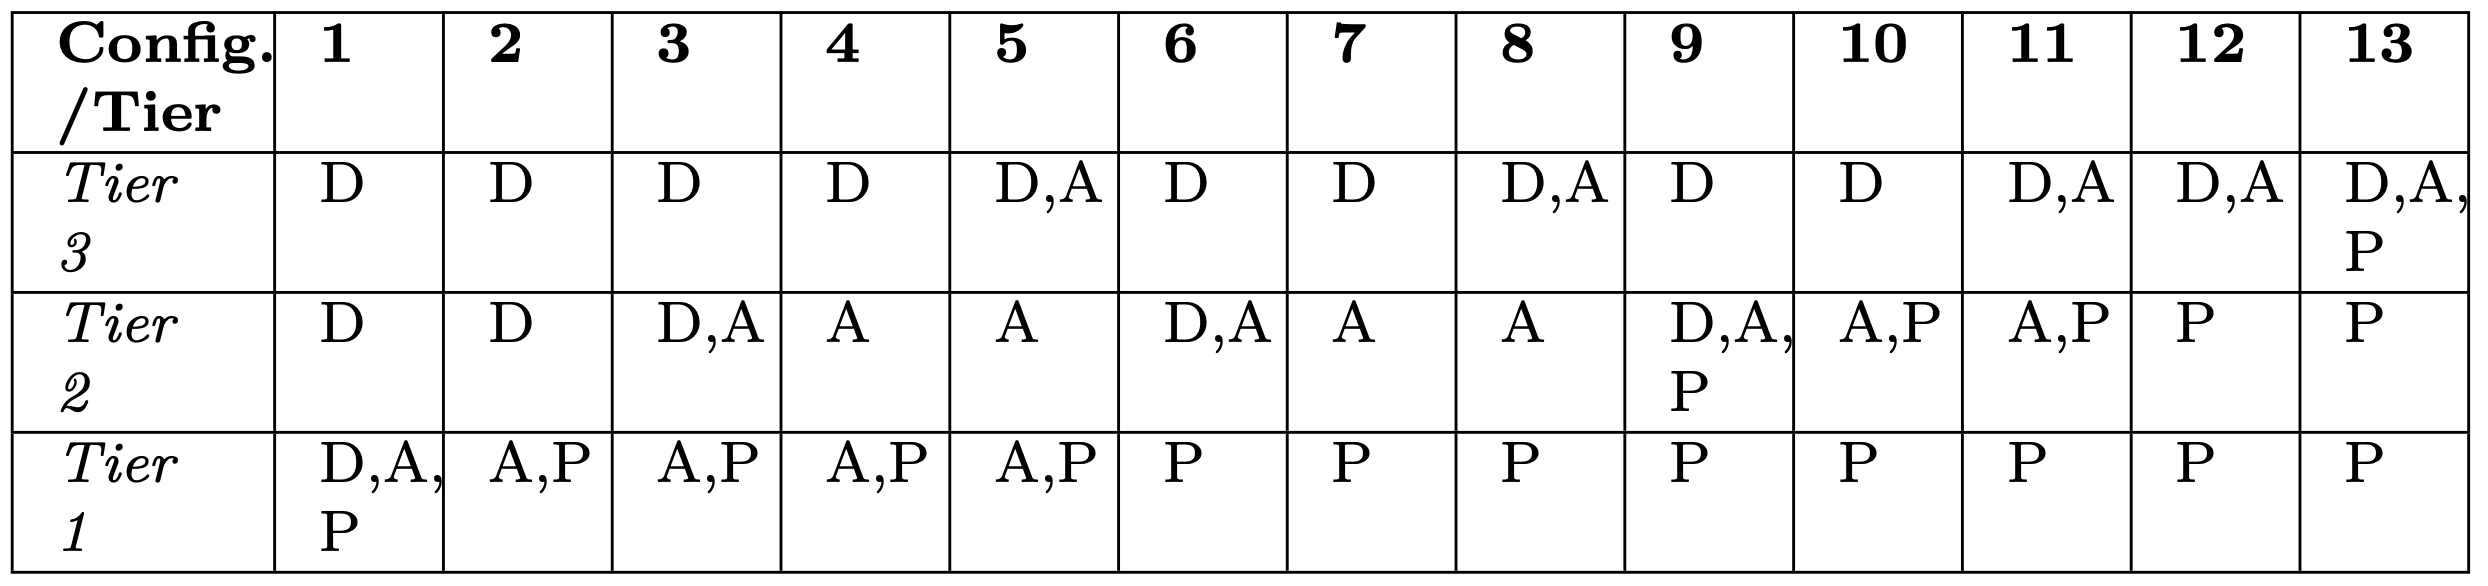
\includegraphics[width=\textwidth]{ClassificationOf3-TierArchitecture}
\centering
\caption{Classification Of 3-Tier Architecture}
\label{fig:Classification Of 3-Tier Architecture}
\end{figure}

By the way, as the Sec.\ref{sec:deployment-view} Deployment View mentioned, we chose the RACS and shared-disk strategy to handle our load balance problem.
In that section, we also proposed two options to deploy our system and why we chose the second option.

\vspace{5mm}

\textbf{Model-View-Controller - MVC}: We referred to the Slide of the Software Engineering 1 course and decided to adopt the MVC pattern to implement our Presentation Layer devices.
As the Fig.\ref{fig:MVC} in Slide showed \cite{SlidesSE1}, the Controller is used to invoke the API and communicate with our Application Server.
The View used to the UI, and the Model used to handle the data arrive from the Application Server and notify the View when something changed.


\begin{figure}[H]
	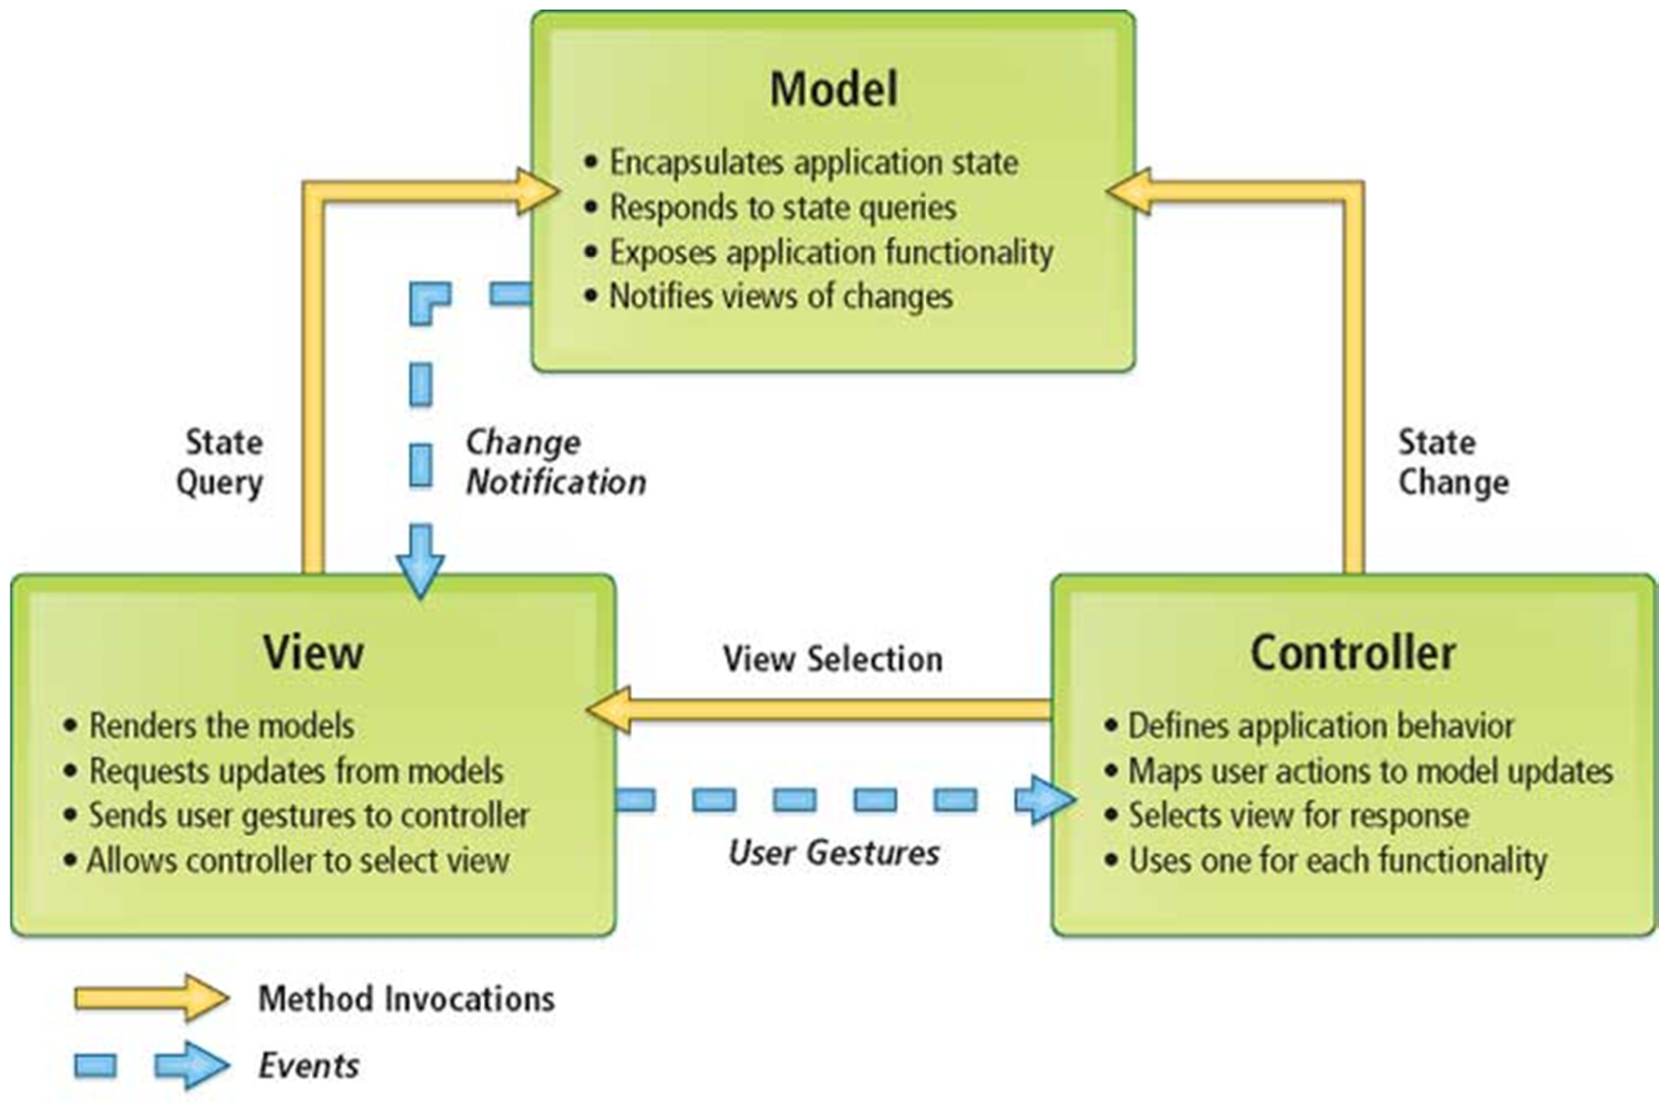
\includegraphics[width=0.7\textwidth]{MVC}
	\centering
	\caption{MVC Pattern}
	\label{fig:MVC}
\end{figure}

\vspace{5mm}

%Observer Pattern
\textbf{Observer Pattern}: We also referred to the observer pattern's idea like the Fig.\ref{fig:Observer Pattern} below in the Slide \cite{SlidesSE1}.
Nevertheless, our system has a specific case: we treat the database as the subject and our CRM component as the Observer.
While some Click Customer's Booking is changed, the CRM will send a notification to the Click Customer Mobile App.
If it is necessary, the CRM will update the E-Ticket for the corresponding customer.

\begin{figure}[H]
	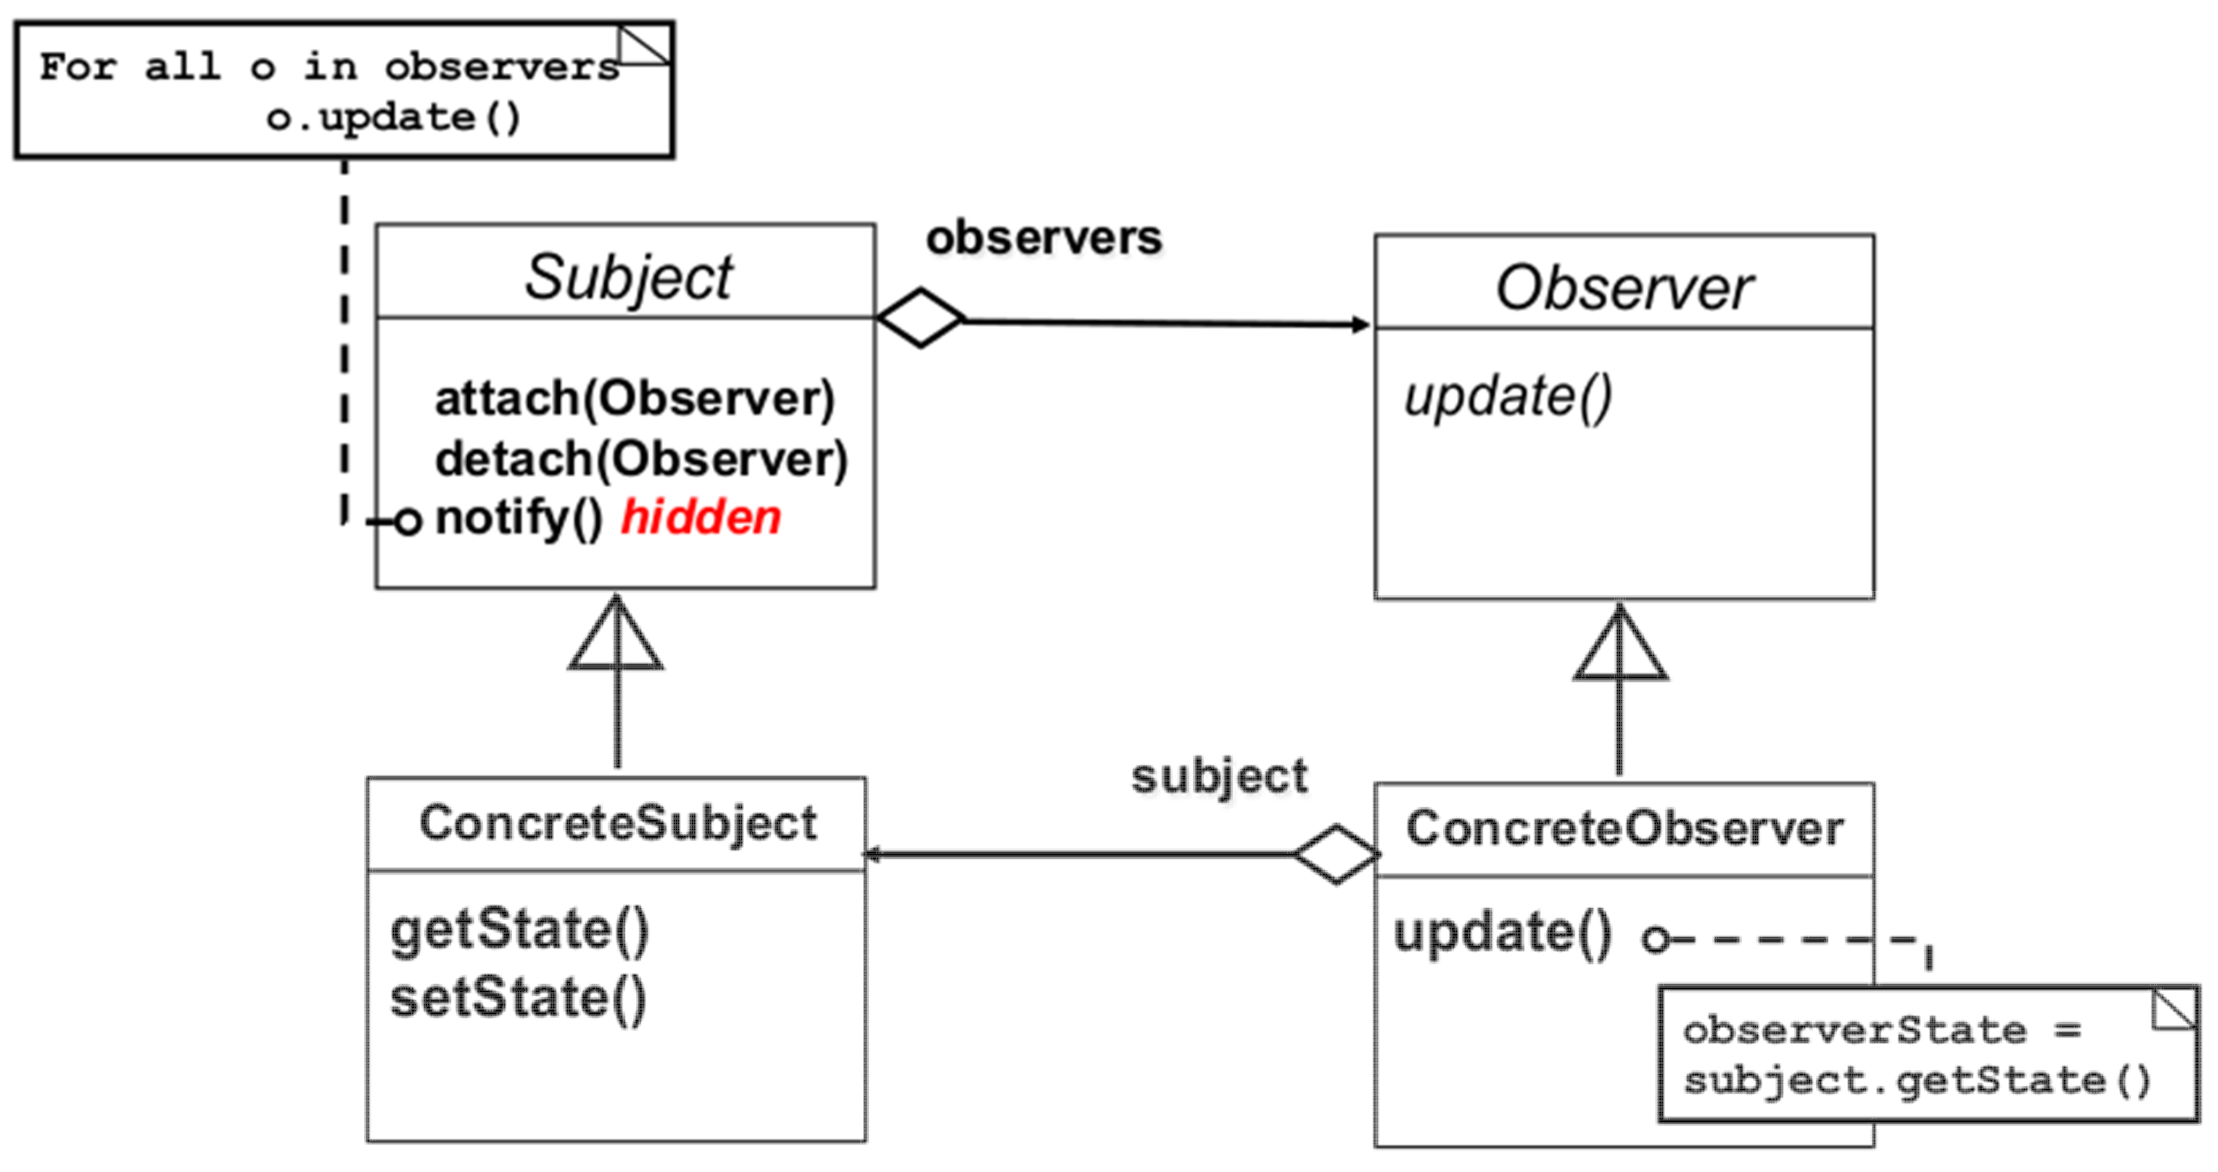
\includegraphics[width=0.7\textwidth]{ObserverPattern}
	\centering
	\caption{Observer Pattern}
	\label{fig:Observer Pattern}
\end{figure}



\section{Other Design Decisions}

In this section, we will talk about the Database Design decision. We referred to the Database 1 Course \cite{Database1Course} and the Database System book \cite{DatabaseSystemBook}.

Our data have several key features: Our data is structured, and the schema can be predefined, and our data structure is vertically scalable instead of horizontally scalable.
So we decided to adopt the \textbf{Relational Database}.

In the database design process, we will strictly follow the design process.
From Conceptual Design to Logical Design, and then to do the Normalization.
Because the Relational Database is vertically scalable, if the initial design is wrong, the cost of later modification will increase exponentially.

For the deployment issues, as the Sec.\ref{sec:deployment-view} Deployment View mentioned, we used \textbf{PostgreSQL} as the Database Management System because it is free, open-source, mature, and stable.



\chapter{USER INTERFACE DESIGN}\label{ch:user-interface-design}

\section{UI design}
We illustrated some main UI designs in RASD document, here, we describe more details for the specific UI design. For every user can use CLup easily and see it clearly, we did the icon and word size bigger, to ensure that even old people can also do it by themselves. ~\\

\subsection{Click Customer Register and Book a Ticket}
For every click customer, they can use their smart phone to download the CLup and book a ticket to the store. The user need to login/register on CLup, after they need to select some shopping details, i.e. date, time, duration time, etc. As shown in following UI design:~\\
~\\ 

\textbf{UI-Date} After enter the booking button, there is an option of date and time, Fig.\ref{fig:UI-Date}, the CLup will give the available booking date, which with the deep dark color. User can choose the date from the available option~\\

\textbf{UI-Time} After user fix the date, they need also select the booking time, as shown in Fig.\ref{fig:UI-Time}, it need to point the AM/PM.~\\

\textbf{UI-DurationTime} It needs the user to estimate his shopping time, Fig.\ref{fig:UI-DurationTime}, for long-term users, the system will also approximate a duration time depending on his shopping history.~\\
~\\
\subsection{Click Customer Get the Ticket}
After the user fulfilled their information, the system will receive their details and schedule the ticket. Users need to wait the notification to inform them that their ticket is ready! After they receive the notification, they can find their E-Ticket in the button of "Ticket". They can with this E-Ticket to enter the store and know the shopping route in the store. As we design in the following:~\\
~\\ 

\textbf{UI-Notification}  Fig.\ref{fig:UI-Notification} which display the user is available, and also inform the user in case of their ticket was rescheduled. The red point means the unread message. The date and time under means the receive message time.

\textbf{UI-TicketBooking}  Fig.\ref{fig:UI-TicketBooking} shows the users available ticket and history tickets. The available ticket with the red point, the time and date under means the booking time(in which time to enter the store). After the user press the PDF icon, they will open the ticket with PDF reader.~\\

\textbf{UI-TicketPDF} The user ticket include 2 pages, the first page Fig.\ref{fig:UI-TicketPDF} display the QRcode using for scan on the entry. And it also give queue number and the suggestion of departing time from current position to the store.~\\

\textbf{UI-Route} This is the second page of user's ticket Fig.\ref{fig:UI-Route} it illustrate the user shopping route in the store. As you can see, in both enter and exit position have the small yellow scan QRCode machine, it needs the user scan-in and scan-out. After, the blue line show the shopping route inside the store, the big yellow cycle point the position of user desired product. The red line show the main map of the store.~\\

\subsection{Brick Customer take the ticket}
For brick customer, they may not available to book the ticket on smart phone. But they can take the ticket on hand-out ticket machine easily. Their ticket will be the same ticket as click customer, also have the QRCode, obviously, brick customer ticket don't need the depart time from home and shopping route, because they've arrived at the store and didn't specific what to buy. Brick customer and click customer all need to wait outside the store, as long as the "Queue number screen" let then go inside. We illustrate some UI design in the following:~\\
~\\
 
\textbf{UI-TakeTicket} It shows the screen of hand-out ticket machine out of the store Fig.\ref{fig:UI-TakeTicket}. Brick customer can take the ticket from here by pressing the "Ticket" button. It will print automatically a PDF ticket to brick customer. It also present the people inside the store and waiting in queue.~\\

\textbf{UI-Queue Number Screen} It displays the screen of queue number orderingFig.\ref{fig:UI-QueueNumberScreen}. This screen shown out of the store, which the user in queue can see it, after they see their corresponding number, they can enter the store with their QRCode.~\\

\subsection{Store Manager management System}
The store manager can control the people density inside the store. In case of too many/less people in the store or in the same zone, he can do three things: (1) He can adjust the max number inside the store. (2) He can reschedule some users' ticket(only users haven't departed yet) (3) He can reschedule the queue order waiting outside the store. We design the manager UI screen in the following:~\\
~\\

\textbf{UI-Reschedule} This displays the screen of manager Fig.\ref{fig:UI-Reschedule}. After the manager press the "Reschedule" button, it will enter to this page, he can smart search for multiple informations. For example, if he saw too many people in the gelato zone, he can search gelato on searching bar, it will show all the Click customers who want to buy gelato, but haven't departed yet. In advanced, he can also smart search the specific time slot of the user, etc. ~\\  

\textbf{UI-Reschedule Click Customer} This displays the screen of manager Fig.\ref{fig:UI-RescheduleCC} for reschedule the click customer. Manager has the right of select users to reschedule their booking time.  As shown is search bar, it display the customer whose deired product is gelato, and the booking time is between 11:30 to 12:00. Manager can press the reschedule button to schedule their booking to another time slot, to reduce the people density in specific store zone. ~\\ 
 
\textbf{UI-Reschedule Queue Order} This describe the screen of manager Fig.\ref{fig:UI-QueueOrder} for reschedule the queue order. Here shown all the arriving customer queue number(Click customer and brick customer). The manager can view the desired product of users, after he can adjust the queue order by showing in queue number screen(we mentioned before).~\\

\begin{figure}[H]
	\begin{minipage}[t]{0.56\linewidth}
		\centering
		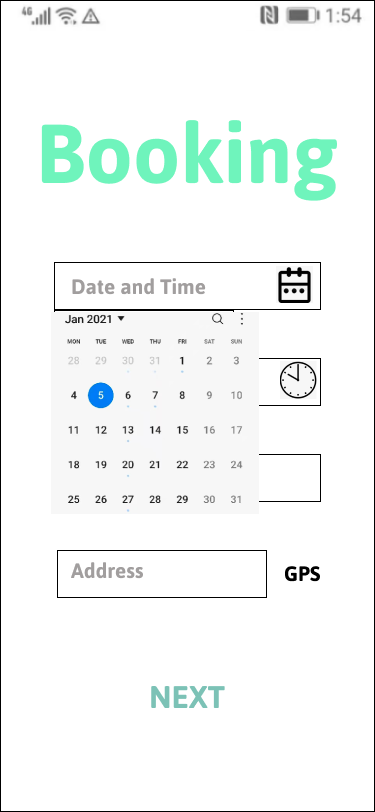
\includegraphics[scale=0.5]{UI-Date.png}
		\caption{UI-Date}
		\label{fig:UI-Date}
	\end{minipage}%
	\begin{minipage}[t]{0.56\linewidth}
		\centering
		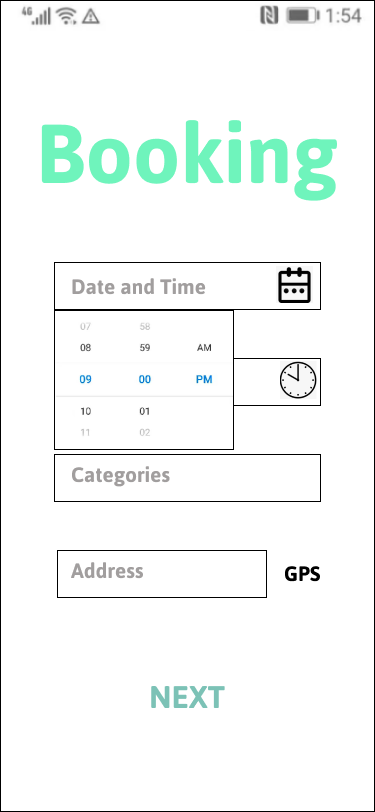
\includegraphics[scale=0.5]{UI-Time.png}
		\caption{UI-Time}
		\label{fig:UI-Time}
	\end{minipage}
\end{figure}

\begin{figure}[H]
	\begin{minipage}[t]{0.56\linewidth}
		\centering
		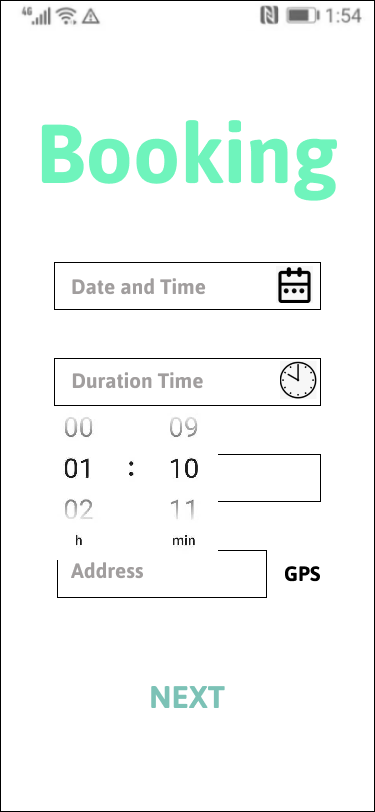
\includegraphics[scale=0.5]{UI-DurationTime.png}
		\caption{UI-DurationTime}
		\label{fig:UI-DurationTime}
	\end{minipage}%
	\begin{minipage}[t]{0.56\linewidth}
		\centering
		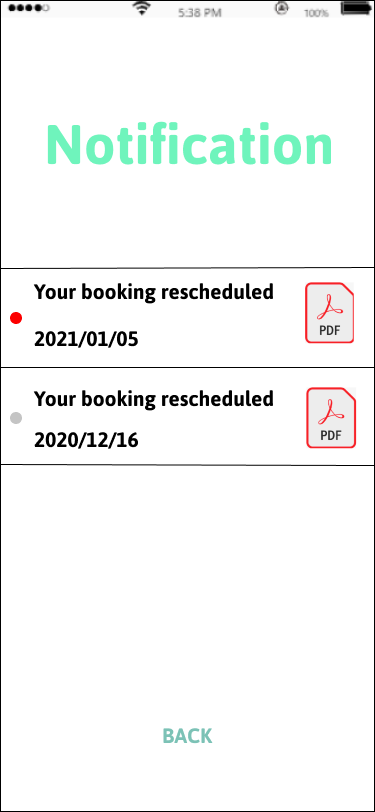
\includegraphics[scale=0.5]{UI-Notification.png}
		\caption{UI-Notification}
		\label{fig:UI-Notification}
	\end{minipage}
\end{figure}

\begin{figure}[H]
	\begin{minipage}[t]{0.56\linewidth}
		\centering
		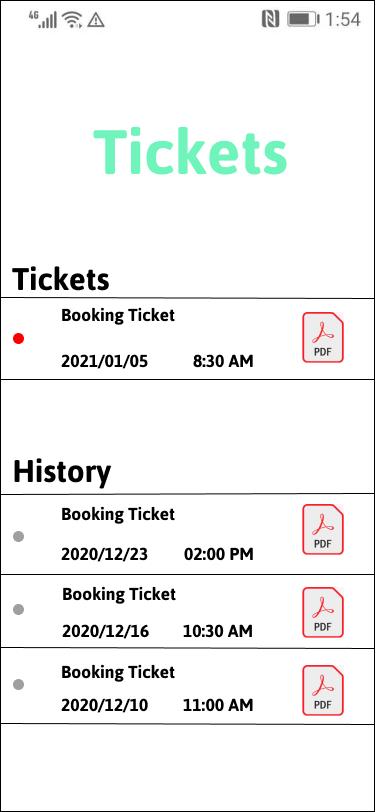
\includegraphics[scale=0.5]{UI-TicketBooking.png}
		\caption{UI-TicketBooking}
		\label{fig:UI-TicketBooking}
	\end{minipage}%
	\begin{minipage}[t]{0.56\linewidth}
		\centering
		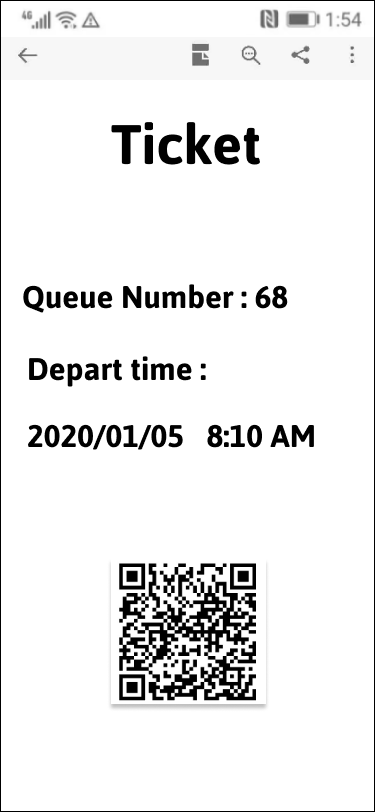
\includegraphics[scale=0.5]{UI-TicketPDF.png}
		\caption{UI-TicketPDF}
		\label{fig:UI-TicketPDF}
	\end{minipage}
\end{figure}

\begin{figure}[H]
	\begin{minipage}[t]{0.56\linewidth}
		\centering
		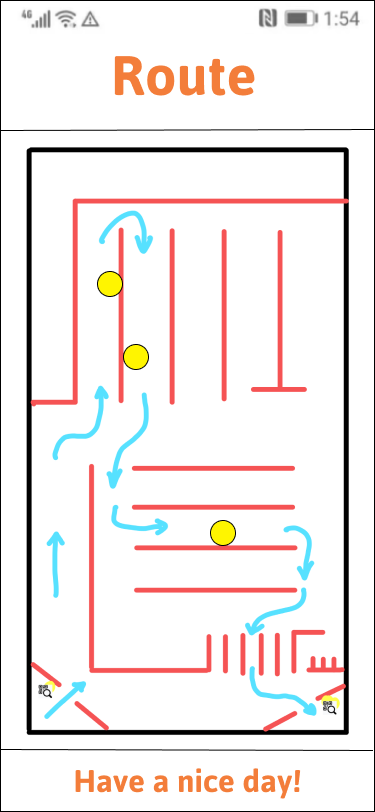
\includegraphics[scale=0.5]{UI-Route.png}
		\caption{UI-Route}
		\label{fig:UI-Route}
	\end{minipage}%
	\begin{minipage}[t]{0.56\linewidth}
		\centering
		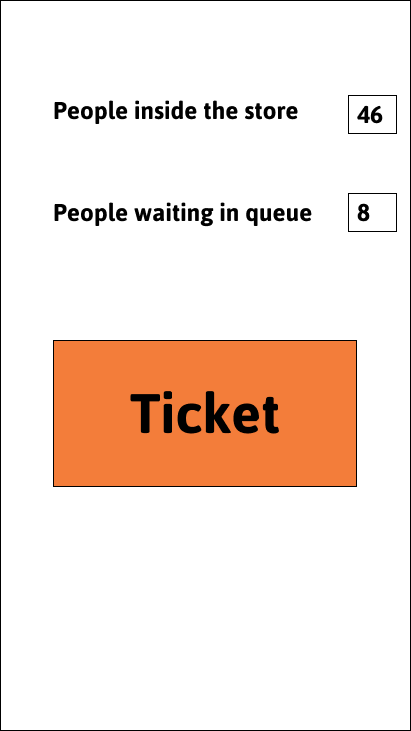
\includegraphics[scale=0.56]{UI-TakeTicket.png}
		\caption{UI-TakeTicket}
		\label{fig:UI-TakeTicket}
	\end{minipage}
\end{figure}


\begin{figure}[H]
	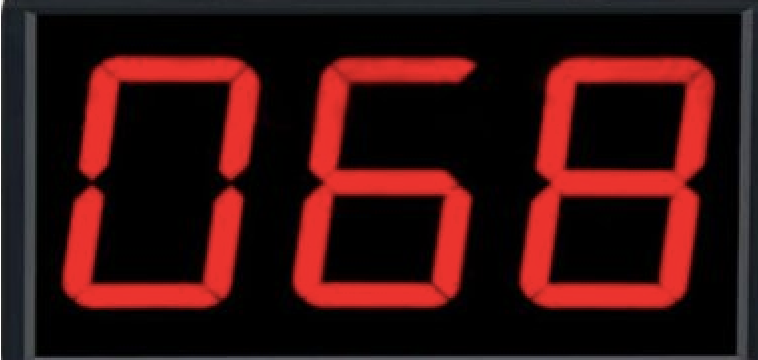
\includegraphics[width=0.56\textwidth]{UI-QueueNumberScreen.png}
	\centering
	\caption{UI-QueueNumberScreen.png}
	\label{fig:UI-QueueNumberScreen}
\end{figure}

\begin{figure}[H]
	\centering
	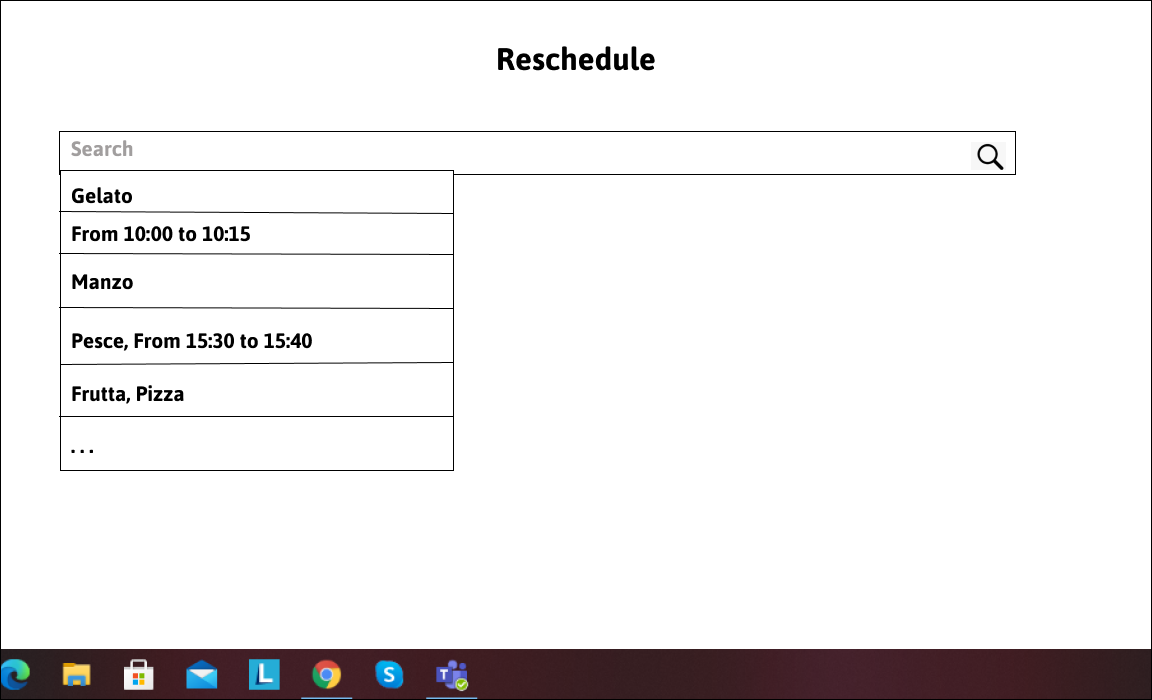
\includegraphics[scale=0.4]{UI-Reschedule.png}
	\caption{UI-Reschedule}
	\centering
	\label{fig:UI-Reschedule}
\end{figure}

\begin{figure}[H]
	\centering
	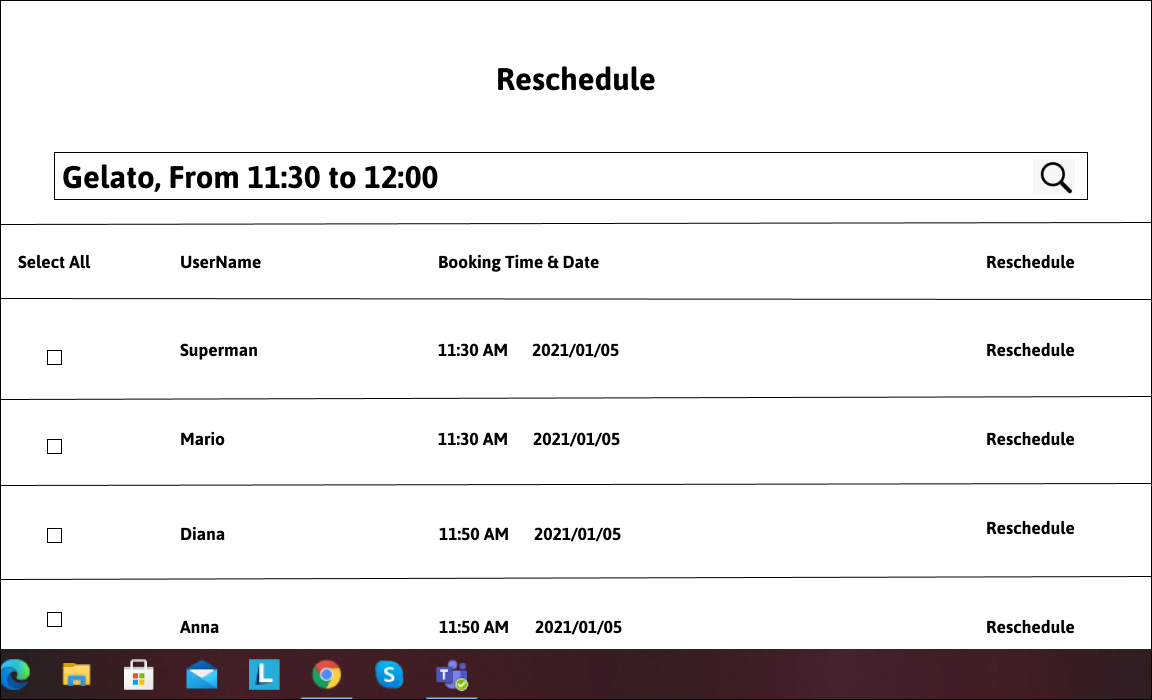
\includegraphics[scale=0.4]{UI-RescheduleCC.png}
	\caption{UI-RescheduleCC}
	\centering
	\label{fig:UI-RescheduleCC}
\end{figure}

\begin{figure}[H]
	\centering
	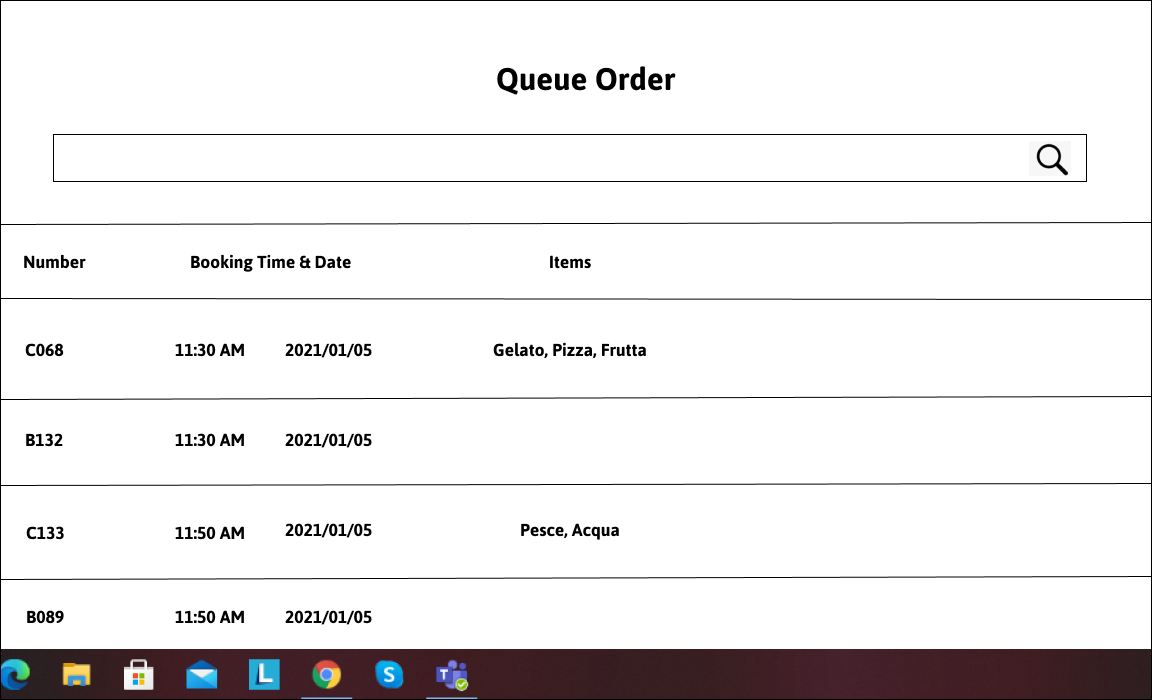
\includegraphics[scale=0.4]{UI-QueueOrder.png}
	\caption{UI-QueueOrder}
	\centering
	\label{fig:UI-QueueOrder}
\end{figure}


\section{UX design}
We present the UX diagram of user, Fig.\ref{fig:ux-user} the diagram show the proceed of how the user from login to get the valid ticket. Corresponding to the UI design, it show the total user view of the CLup application. Of course we cannot show all the details the user proceed, we pick the main point to illustrate the UX for user. And we also add some character aiming to complete the UX, e.t."Logout", which we didn't mention in RASD~\\


\begin{figure}[H]
	\centering
	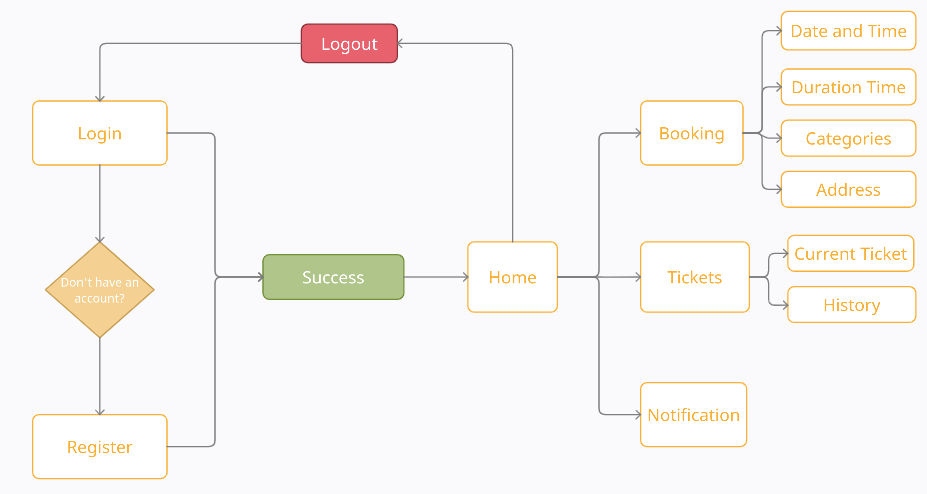
\includegraphics[scale=0.5]{UX-User}
	\caption{UX-User}
	\centering
	\label{fig:ux-user}
\end{figure}



\chapter{REQUIREMENTS TRACEABILITY}\label{ch:requirements-traceability}

In this chapter, we will bind the Goals specified in RASD with the component in DD.

\section{G1 : Allows store managers to regulate the influx of people in the building}
\subsection{Requirements}
\begin{itemize}
	\item $R_7$: The Store Manager shall be able to Check out the On-Time Store Data.
	\item $R_8$: The Store Manager shall be able to Adjust the maximum number of people in the store.
	\item $R_9$: The Store Manager shall be able to Adjust the order of the queue.
	\item $R_{10}$: The Store Manager shall be able to Check and reschedule the booking.
	\item $R_{12}$: The Store Back-End System shall be able to received and schedule the click customers' booking. The scheduling must refer to the duration time of each Customer and the categories of items that the Customer intends to buy.
	\item $R_{15}$: The Store Back-End System shall send a notification and update the E-Ticket to the Customer when their book is rescheduled.
	\item $R_{17}$: The Store Back-End System shall analyze the historical visit data and calculate the average history duration for the Long-Term Customers.
	\item $R_{18}$: The Store Back-End System shall be able to Calculate and store the On-Time Store Data.
	\item $R_{19}$: The Store Back-End System shall schedule or reschedule the queue order from click customer's booking and the brick customer's retrieved ticket.
	\item $R_{20}$: The Store Back-End System shall be able to Control the Digital Counterpart and display the queue number.
	\item $R_{21}$: The Store Back-End System shall be able to receive the information from the QR Code Scanned Machine. Receive the information from the Tickets Hand-Out Machine.
\end{itemize}

\subsection{Domain Assumptions}
\begin{itemize}
	\item $D_4$ : If something unexpected happens, the store manager can reasonably adjust the maximum number of people in the store or reschedule the queue \& Customer's book.
	\item $D_5$ : If someone's booking is rescheduled, he can find the notification in time and set off according to the updated E-Ticket.
\end{itemize}

\subsection{Components}
\begin{itemize}
	\item $C_1$: CRM
	\item $C_2$: QueueSchedule
	\item $C_3$: BookingSchedule
	\item $C_4$: ClickCustomerMobileApp
	\item $C_5$: DigitalCounterpart
	\item $C_6$: TicketHandOutMachine
	\item $C_7$: QRCodeScannedMachine
	\item $C_{8}$: StoreManagerManagementSystem
	\item $C_{9}$: DBMSServer
\end{itemize}


\section{$G_2$ : Saves people from having to line up and stand outside of stores for hours on end}

\subsection{Requirements}

\begin{itemize}
	\item $R_1$: Each Click Customer shall be able to sign-up and Log-in.
	\item $R_2$: Each Click Customer shall be able to book a visit.
	\item $R_3$: Each Click Customer shall be able to check on the E-Ticket.
	\item $R_4$: Each Click Customer shall check on the store manager's notification when their book is rescheduled.
	\item $R_5$: Each Brick Customer shall be able to retrieve the Ticket from the Tickets Hand-Out Machine and wait for the Digital Counterpart to call them.
	\item $R_6$: Each Customer shall scan the QR Code at QR Code scanned machine when they enter and leave the store.
	\item $R_{11}$: The Store Back-End System shall send the available time/date to the click customers.
	\item $R_{12}$: The Store Back-End System shall be able to received and schedule the click customers' booking. The scheduling must refer to the duration time of each Customer and the categories of items that the Customer intends to buy.
	\item $R_{13}$: The Store Back-End System shall calculate the time from the click customer's departure place to the store and put the estimated departure time on the E-Ticket.
	\item $R_{15}$: The Store Back-End System shall send a notification and update the E-Ticket to the Customer when their book is rescheduled.
	\item $R_{16}$: The Store Back-End System shall be able to store the Customer's data.
	\item $R_{17}$: The Store Back-End System shall analyze the historical visit data and calculate the average history duration for the Long-Term Customers.
	\item $NR_1$:The time from the click customer's departure place to the store that calculates from the Store Back-End System must be precise enough to avoid the Customer arriving at the store too early/late.
	\item $NR_2$:The Store Back-End System must schedule the queue reasonably to minimize the wait time.
	\item $NR_3$:The Store Back-End System must mix the book and brick customer's retrieved ticket reasonably to allow the click customers to enter the store near the book time by avoiding making the brick customers wait too long.
	\item $NR_4$:Cause everyone needs to do grocery shopping, the software for the click customer should be simple enough to use.
\end{itemize}


\subsection{Domain Assumptions}

\begin{itemize}
	\item $D_1$ : Everyone will leave the departure place at the departure time indicated by the system.
	\item $D_2$ : Everyone who leaves on time can arrive at the store on time.
	\item $D_3$ : After shopping, everyone can leave the store in time according to their estimated time.
	\item $D_5$ : If someone's booking is rescheduled, he can find the notification in time and set off according to the updated E-Ticket.
	\item $D_6$ : Everyone can consciously scan the QR code at the entrance and exit.
	\item $D_8$ : If possible, everyone tries to book the visit via the application(be a \hyperref[Definitions]{Click Customer}) instead of picking up tickets on the spot(not be a \hyperref[Definitions]{Brick Customer}).
\end{itemize}


\subsection{Components}
\begin{itemize}
	\item $C_1$: CRM
	\item $C_2$: QueueSchedule
	\item $C_3$: BookingSchedule
	\item $C_4$: ClickCustomerMobileApp
	\item $C_5$: DigitalCounterpart
	\item $C_6$: TicketHandOutMachine
	\item $C_7$: QRCodeScannedMachine
	\item $C_{9}$: DBMSServer
	\item $C_{10}$: GoogleMap Service
\end{itemize}


\section{$G_3$ : The application plan visits in a finer way to allow more people in the store, at the same time, let the customer occupy different spaces in the store to keep enough distance between them}

\subsection{Requirements}

\begin{itemize}
	\item $R_{12}$: The Store Back-End System shall be able to received and schedule the click customers' booking. The scheduling must refer to the duration time of each Customer and the categories of items that the Customer intends to buy.
	\item $R_{14}$: The Store Back-End System shall Plan and put the Store Planned Roadmap on the E-Ticket Send the E-Ticket to the click customers.
	\item $R_{17}$: The Store Back-End System shall analyze the historical visit data and calculate the average history duration for the Long-Term Customers.
\end{itemize}

\subsection{Domain Assumptions}

\begin{itemize}
	\item $D_3$ : After shopping, everyone can leave the store in time according to their estimated time.
	\item $D_7$ : Everyone can follow the \hyperref[Definitions]{Planned Roadmap} in the store.
\end{itemize}

\subsection{Components}

\begin{itemize}
	\item $C_1$: CRM
	\item $C_3$: BookingSchedule
	\item $C_4$: ClickCustomerMobileApp
	\item $C_{9}$: DBMSServer
\end{itemize}



%\begin{center}
%	\begin{tabular}{ |c|c|c| }
%		\hline
%		
%
%	\end{tabular}
%\end{center}

\chapter{IMPLEMENTATION, INTEGRATION AND TEST PLAN}\label{ch:implementation-integration-and-test-plan}


\section{Implementation }
We use the Top-down design approach. When a click customer want to book a ticket, the following modules will be implemented is this order:~\\
~\\
$\bullet$ ClickCustomerMobileApp~\\
$\bullet$ Redirector~\\
$\bullet$ CRM~\\
$\bullet$ BookingSchedule~\\
$\bullet$ DBMSServer~\\
~\\
For the store manager management system, the modules sequence is this:~\\
~\\
$\bullet$ StoreManagerManagementSystem~\\
$\bullet$ Redirector~\\
$\bullet$ QueueSchedule~\\
$\bullet$ BookingSchedule~\\
$\bullet$ DBMSServer~\\


\section{Integration}
The aiming od integration testing is at exercising: interface and modules interactions. We need to consider and avoid the different integration faults:~\\
~\\
$\bullet$ Side effects on parameters or resources~\\
$\bullet$ Violations of value domains, capacity, or size limits~\\
$\bullet$ Omitted or misunderstood functionality~\\
$\bullet$ Nonfunctional properties~\\
$\bullet$ Dynamic mismatches\cite{SlidesSE2}~\\
~\\
Our integration testing based on the Top-down structure of system with the thread of a portion of several modules offers a user- visible function.~\\
~\\
\section{Test Plan}
We will use the black-box testing. We will use modules to devise test cases, and the actural behavior of software under test is checked against the the behavior specified by the model. The prerequisties of performances testing is expected workload and acceptable performance. For system testing, the teams are independent and will test the functional and non-functional requirements. As for the test environment, it need to be as close as possiable to production enviroment. In performance, we need to identify the inefficient algorithms, optimize the query possibilities and hardware/ network issues\cite{SlidesSE2}.



\chapter{Effort Spent}

\begin{itemize}
	\item \textbf{Kong XiangYi}
	\begin{center}
		\scalebox{0.8}{
			\begin{tabular}{ |c|c|c| }
				\hline
				Date & Task & Hours \\
				\hline
				\hline
				2021/01/02 & Group discussion and task assignment & 2h \\
				\hline
				2021/01/04 & UI design & 2h \\
				\hline
				2021/01/05 & UX design diagram in chapter 3& 2h \\
				\hline
				2021/01/06 & Complete UI and UX design in chapter 3& 5h \\
				\hline
				2021/01/07 &  Did chapter 5 implementation, integrate and test & 4h \\
				\hline
				2021/01/08 & Group Discussion & 2h\\
				\hline
				2021/01/08 & Did the chapter 1 and chapter 5 & 3h\\
				\hline

		\end{tabular}}
	\end{center}


	\item \textbf{Zhang YueDong}
	\begin{center}
		\scalebox{0.8}{
			\begin{tabular}{ |c|c|c| }
				\hline
				Date & Task & Hours \\
				\hline
				\hline
				2021/01/01 &  Launch DD  & 2h \\
				\hline
				2021/01/02 & Group discussion and task assignment & 2h \\
				\hline
				2021/01/03 & Did S.\ref{ch:architectural-design}.\ref{sec:ArchitectureOverview}
				and S.\ref{ch:architectural-design}.\ref{sec:ComponentView}
				Component Diagram & 3h \\
				\hline
				2021/01/04 & Did S.\ref{sec:ComponentView}.
				Component Diagram describe. & 2h \\
				\hline
				2021/01/05 & Did S.\ref{sec:deployment-view}.
				Deployment Diagram and describe. & 5h \\
				\hline
				2021/01/06 & Did S.\ref{sec:RuntimeViwe}.
				Runtime View and describe & 4h \\
				\hline
				2021/01/07 & Did S.\ref{sec:component-interfaces}.
				Component Interface describe & 2h \\
				\hline
				2021/01/08 & Finished the architecture part and did the group discussion. & 4h \\
				\hline
			\end{tabular}}
	\end{center}
\end{itemize}




%Bibliographic references
\begin{thebibliography}{9}

\bibitem{SistemiInformativi}
Cinzia Cappiello, Mariagrazia Fugini, Paul Grefen, Barbara Pernici, Pierluigi Plebani, Monica Vitali. (7 settembre 2018)  \textbf{Fondamenti di Sistemi informativi}: per il Settore dell'Informazione.

\bibitem{IEEESDD}
"IEEE Standard for Information Technology--Systems Design--Software Design Descriptions," in IEEE STD 1016-2009 , vol., no., pp.1-35, 20 July 2009, doi: 10.1109/IEEESTD.2009.5167255.

\bibitem{IEEEAD}
"ISO/IEC/IEEE Systems and software engineering -- Architecture description," in ISO/IEC/IEEE 42010:2011(E) (Revision of ISO/IEC 42010:2007 and IEEE Std 1471-2000) , vol., no., pp.1-46, 1 Dec.
2011, doi: 10.1109/IEEESTD.2011.6129467.

\bibitem{SlidesSE1}
Gianpaolo Cugola, Lorenzo Di Tucci. (A.Y.2018/2019) The slides of the Software Engineering 1 course.
Politecnico di Milano.

\bibitem{SlidesSE2}
Elisabetta Di Nitto, Matteo Rossi. (A.Y.2020/2021) The slides of the Software Engineering 2 course.
Politecnico di Milano.

\bibitem{Database1Course}
Sara Comai, Giovanni Meroni, Davide Piantella. (A.Y.2019/2020) The Database 1 course.
Politecnico di Milano.

\bibitem{DatabaseSystemBook}
Paolo Atzeni, Stefano Ceri, Stefano Paraboschi, Riccardo Torlone. \textbf{Database Systems} concepts, languages \& architectures.
The McGraw-Hill Companies.
ISBN 007-709500-6.


\end{thebibliography}


\end{document}

